\newpage\section{Arrowhead Matrix Visualization}

This section presents the application of the orthogonal vector generation techniques to visualize arrowhead matrices and their eigenvalues and eigenvectors. The arrowhead matrix is a special type of matrix with non-zero elements only in the first row, first column, and along the diagonal.

\subsection{Arrowhead Matrix Structure and Creation Process}

An arrowhead matrix has the following structure:

\begin{equation}
A = 
\begin{pmatrix}
a & b_1 & b_2 & \cdots & b_n \\
b_1 & c_1 & 0 & \cdots & 0 \\
b_2 & 0 & c_2 & \cdots & 0 \\
\vdots & \vdots & \vdots & \ddots & \vdots \\
b_n & 0 & 0 & \cdots & c_n
\end{pmatrix}
\end{equation}

In our implementation, we generate arrowhead matrices using orthogonal vectors created in the plane perpendicular to the x=y=z line. We use 72 theta steps (0 to 360 degrees in 5-degree increments) to generate a smooth visualization of the matrices and their properties. The creation process involves the following steps:

\begin{enumerate}
    \item Generate an orthogonal vector $R$ by varying the $\theta$ parameter, which creates a circle in the plane orthogonal to the x=y=z line using the basis vectors [1, -1/2, -1/2] and [0, -1/2, 1/2].
    \item Extract the three components of the R vector: $R_0$ (x component), $R_1$ (y component), and $R_2$ (z component).
    \item Calculate potential functions for each component:
    \begin{itemize}
        \item $V_X(R)$: A parabolic potential function $0.5 \cdot x^2$
        \item $V_A(R)$: A shifted parabolic potential function $0.5 \cdot (x-1)^2$
    \end{itemize}
    \item Construct the diagonal elements of the matrix:
    \begin{itemize}
        \item First diagonal element ($D_{00}$): Sum of all $V_X$ potentials plus $\hbar\omega$
        \item Second diagonal element ($D_{11}$): $V_A(R_0) + V_X(R_1) + V_X(R_2)$
        \item Third diagonal element ($D_{22}$): $V_X(R_0) + V_A(R_1) + V_X(R_2)$
        \item Fourth diagonal element ($D_{33}$): $V_X(R_0) + V_X(R_1) + V_A(R_2)$
    \end{itemize}
    \item Set all off-diagonal elements in the first row and first column to a coupling constant of 0.1, representing interactions between elements.
\end{enumerate}

This process creates a 4×4 arrowhead matrix where the diagonal elements vary based on the potential functions and the $\theta$ parameter, while the off-diagonal elements (the "arrows") have a fixed coupling value of 0.1.

\subsection{Example Arrowhead Matrix}

Below is an example of a 4×4 arrowhead matrix generated with $\theta = 45^{\circ}$, with values taken directly from the CSV file \texttt{arrowhead\_matrix\_4x4\_theta\_45.csv}:

\begin{equation}
A_{\theta=45^{\circ}} = 
\begin{pmatrix}
0.042 & 0.1 & 0.1 & 0.1 \\
0.1 & 0.830 & 0 & 0 \\
0.1 & 0 & 0.542 & 0 \\
0.1 & 0 & 0 & 0.542
\end{pmatrix}
\end{equation}

This matrix has a coupling value of 0.1 in the off-diagonal elements, representing the interaction between the first element and all other elements in the system.

\subsection{Eigenvalue Visualization}

The eigenvalues of the arrowhead matrices are calculated for different values of $\theta$ ranging from 0° to 355° in 5° increments. This creates a pattern of eigenvalues that can be visualized in both 2D and 3D.

\subsubsection{2D Eigenvalue Plots}

Figure \ref{fig:all_eigenvalues_2d} shows the eigenvalues of the arrowhead matrices plotted against the $\theta$ parameter. Each eigenvalue is represented by a different color.

\begin{figure}[H]
    \centering
    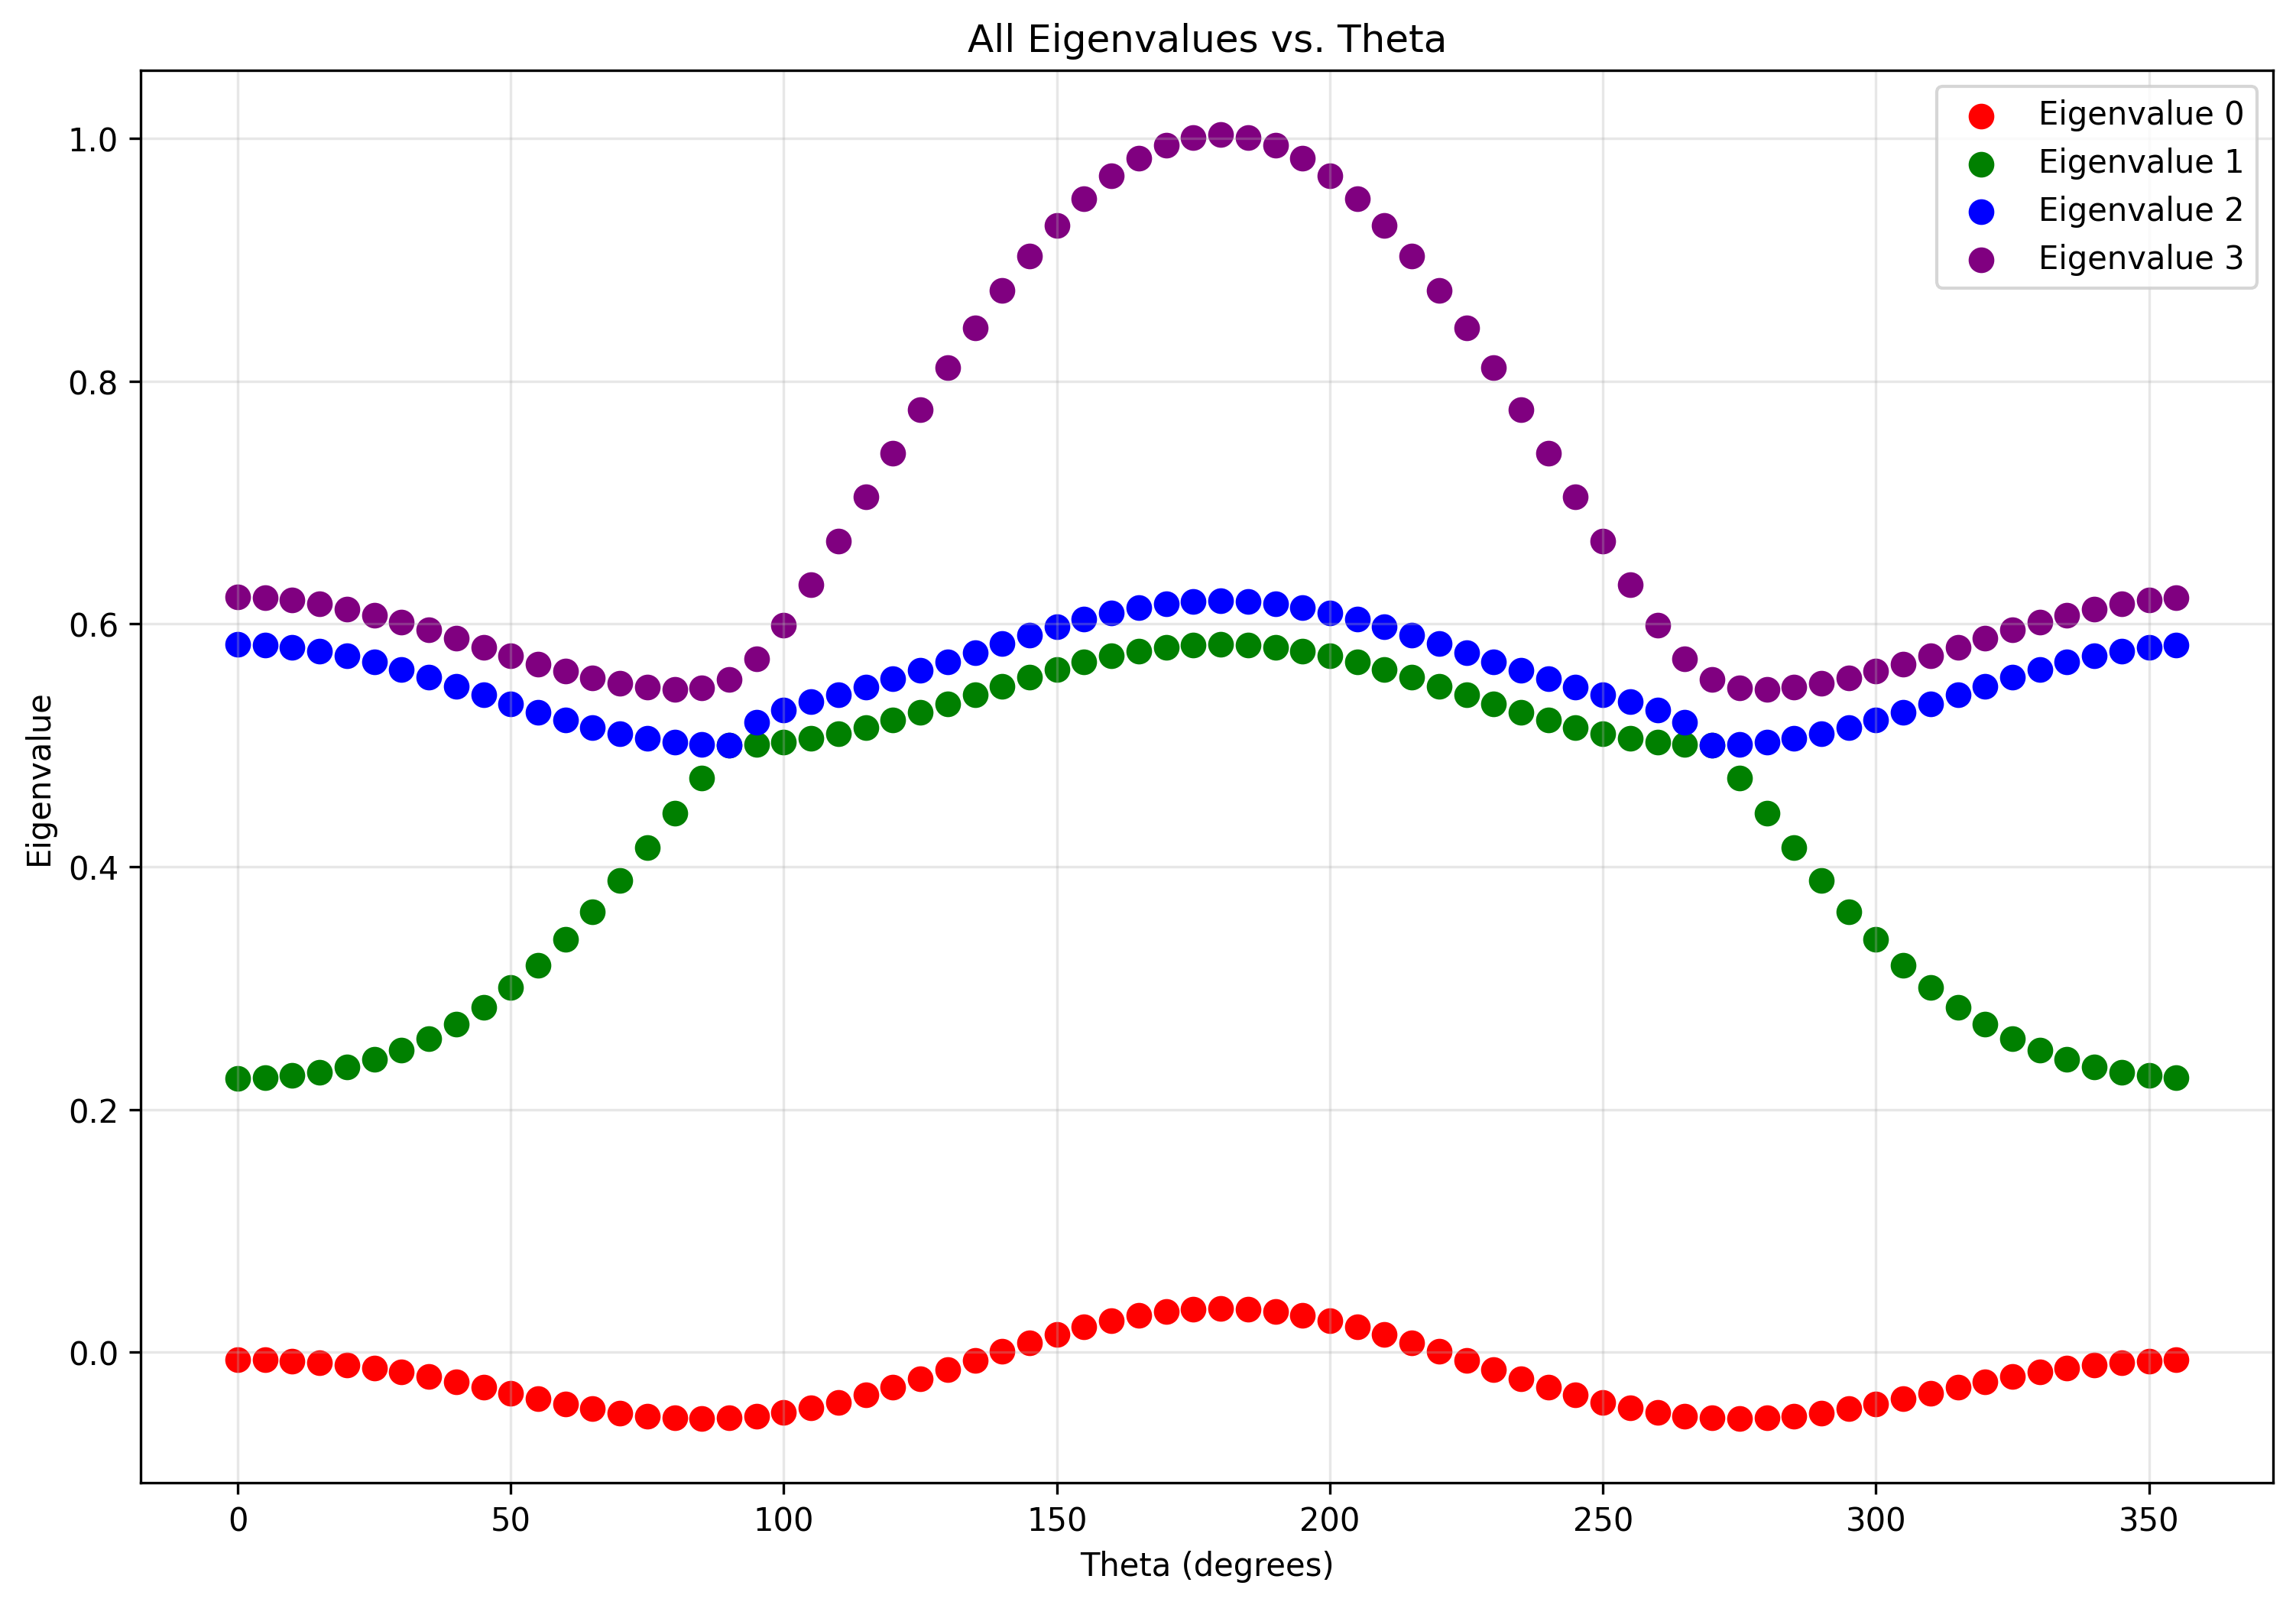
\includegraphics[width=0.8\textwidth]{../example_use/arrowhead_matrix/results/plots/all_eigenvalues_2d.png}
    \caption{All eigenvalues plotted against $\theta$}
    \label{fig:all_eigenvalues_2d}
\end{figure}

Individual plots for each eigenvalue are also generated to provide a clearer view of how each eigenvalue changes with $\theta$. Figures \ref{fig:eigenvalue_0_2d} through \ref{fig:eigenvalue_3_2d} show the plots for each eigenvalue.

\begin{figure}[H]
    \centering
    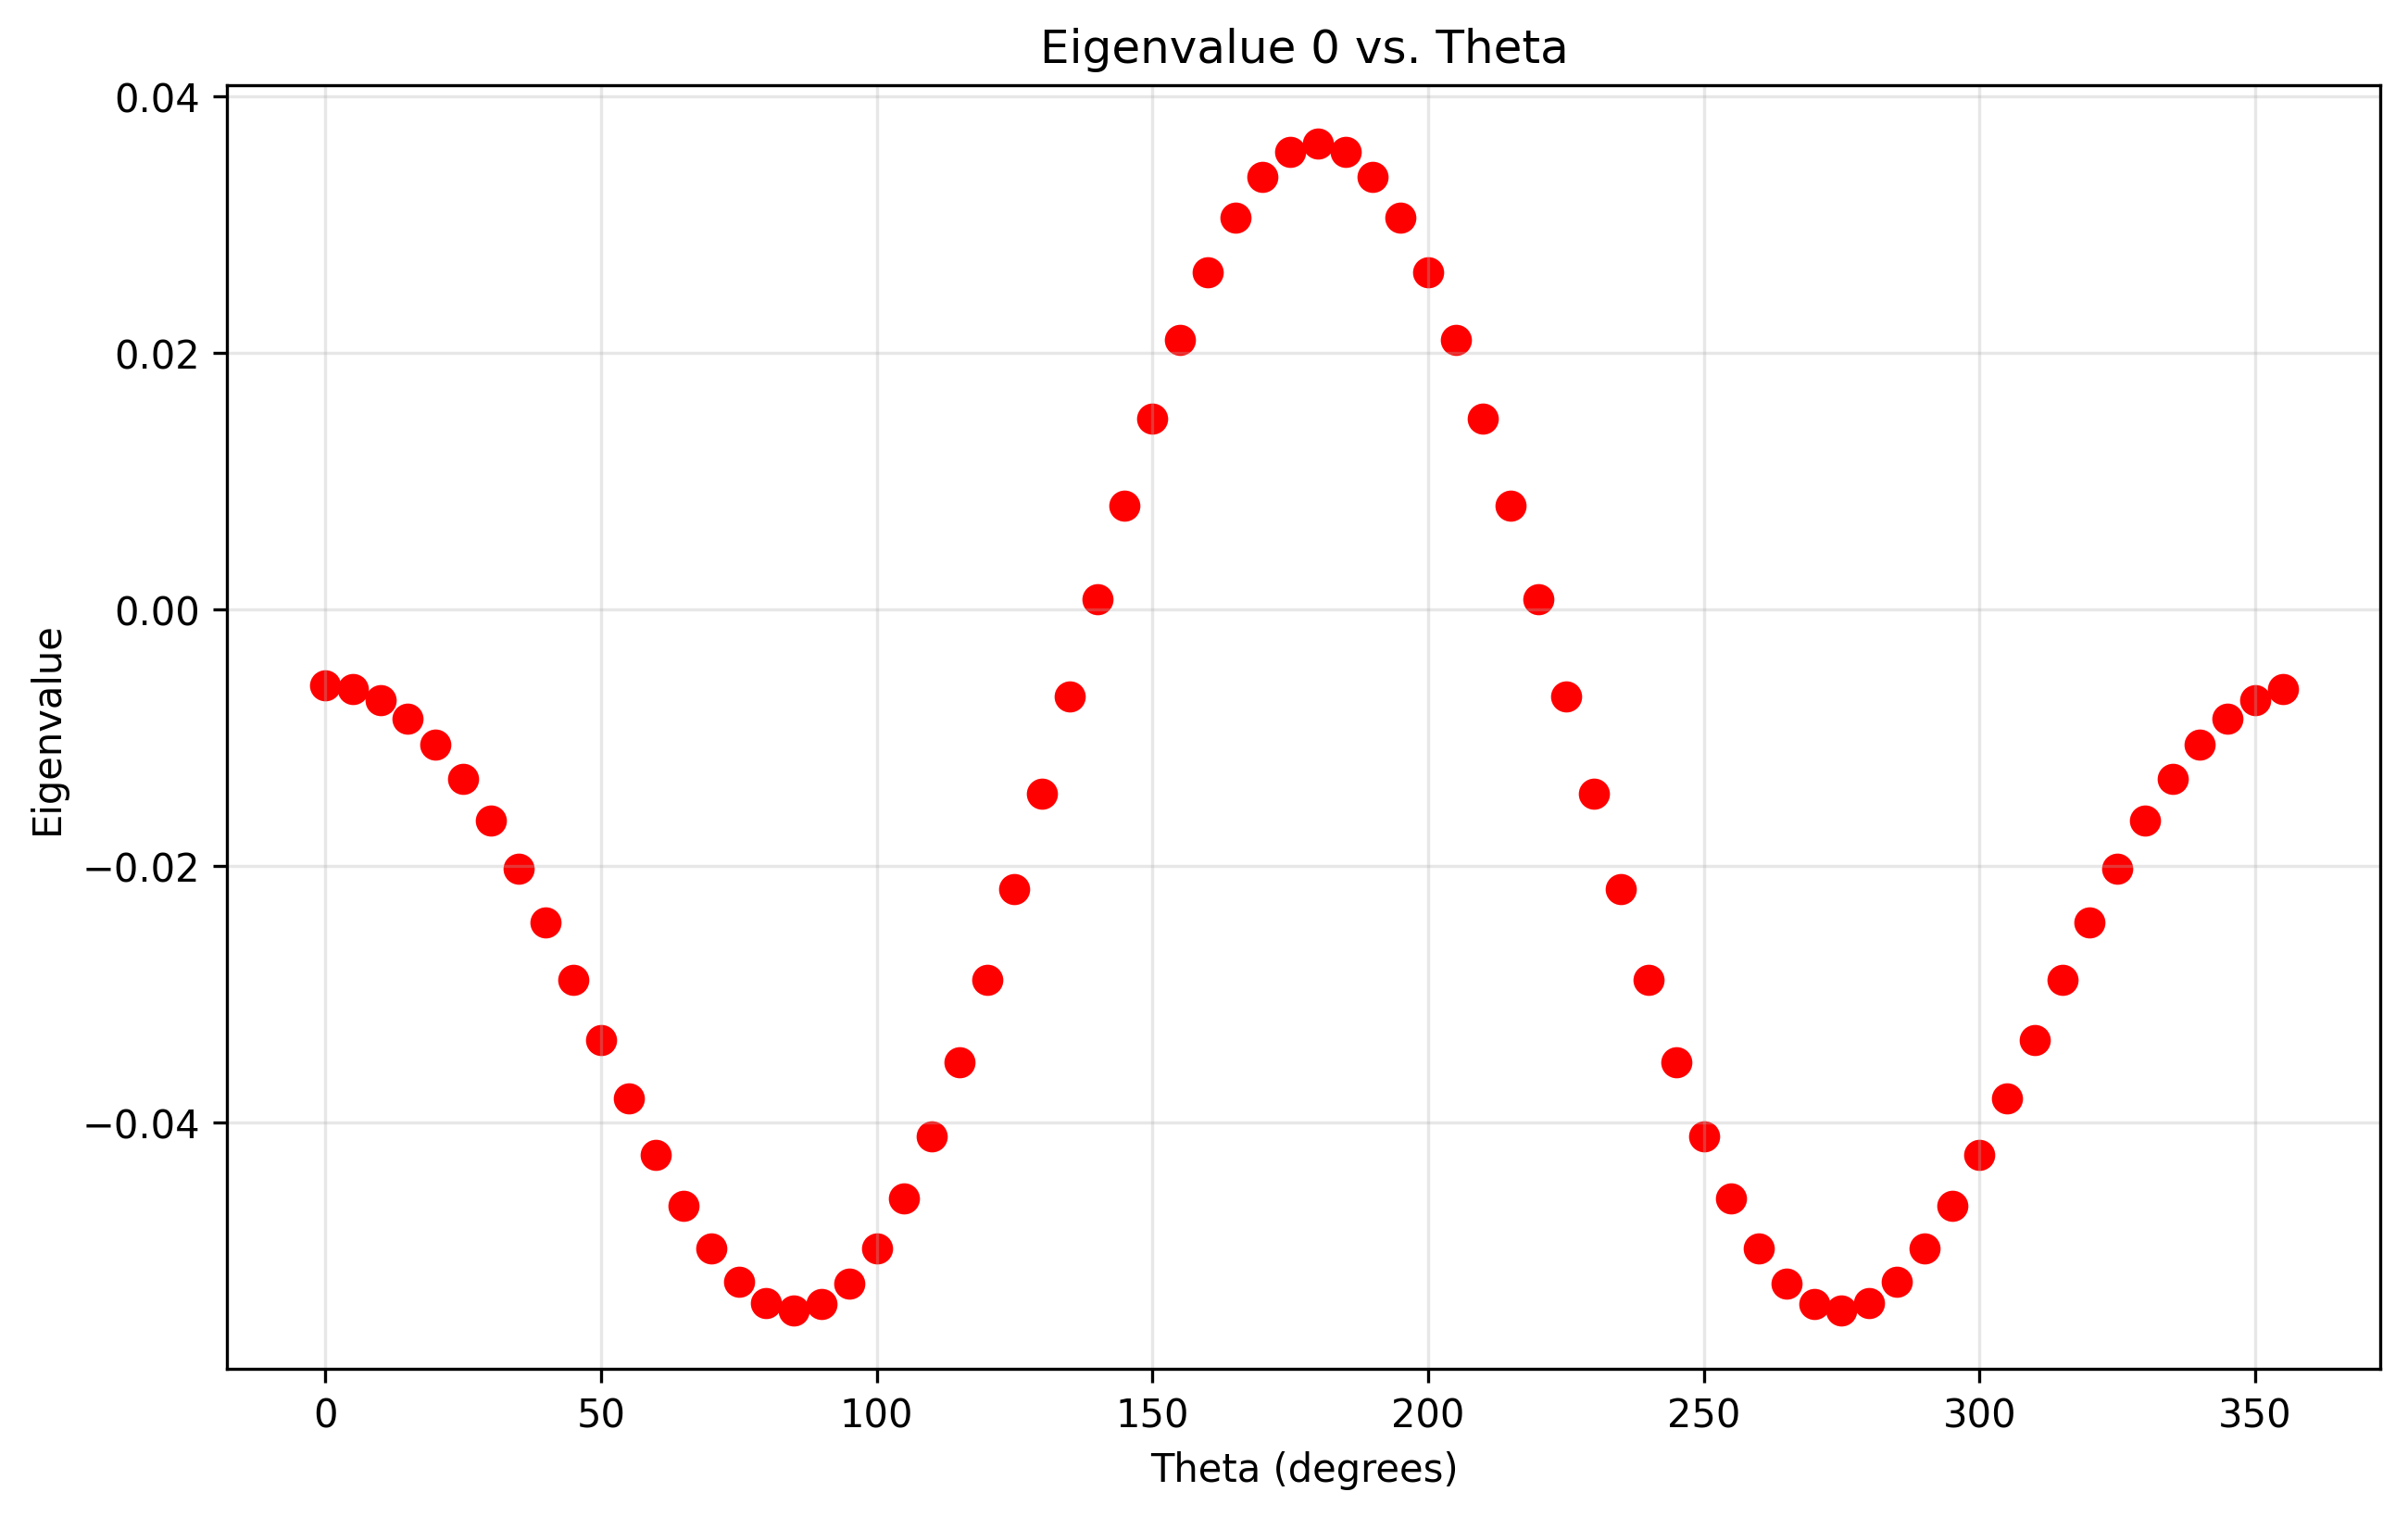
\includegraphics[width=0.8\textwidth]{../example_use/arrowhead_matrix/results/plots/eigenvalue_0_2d.png}
    \caption{First eigenvalue plotted against $\theta$}
    \label{fig:eigenvalue_0_2d}
\end{figure}

\begin{figure}[H]
    \centering
    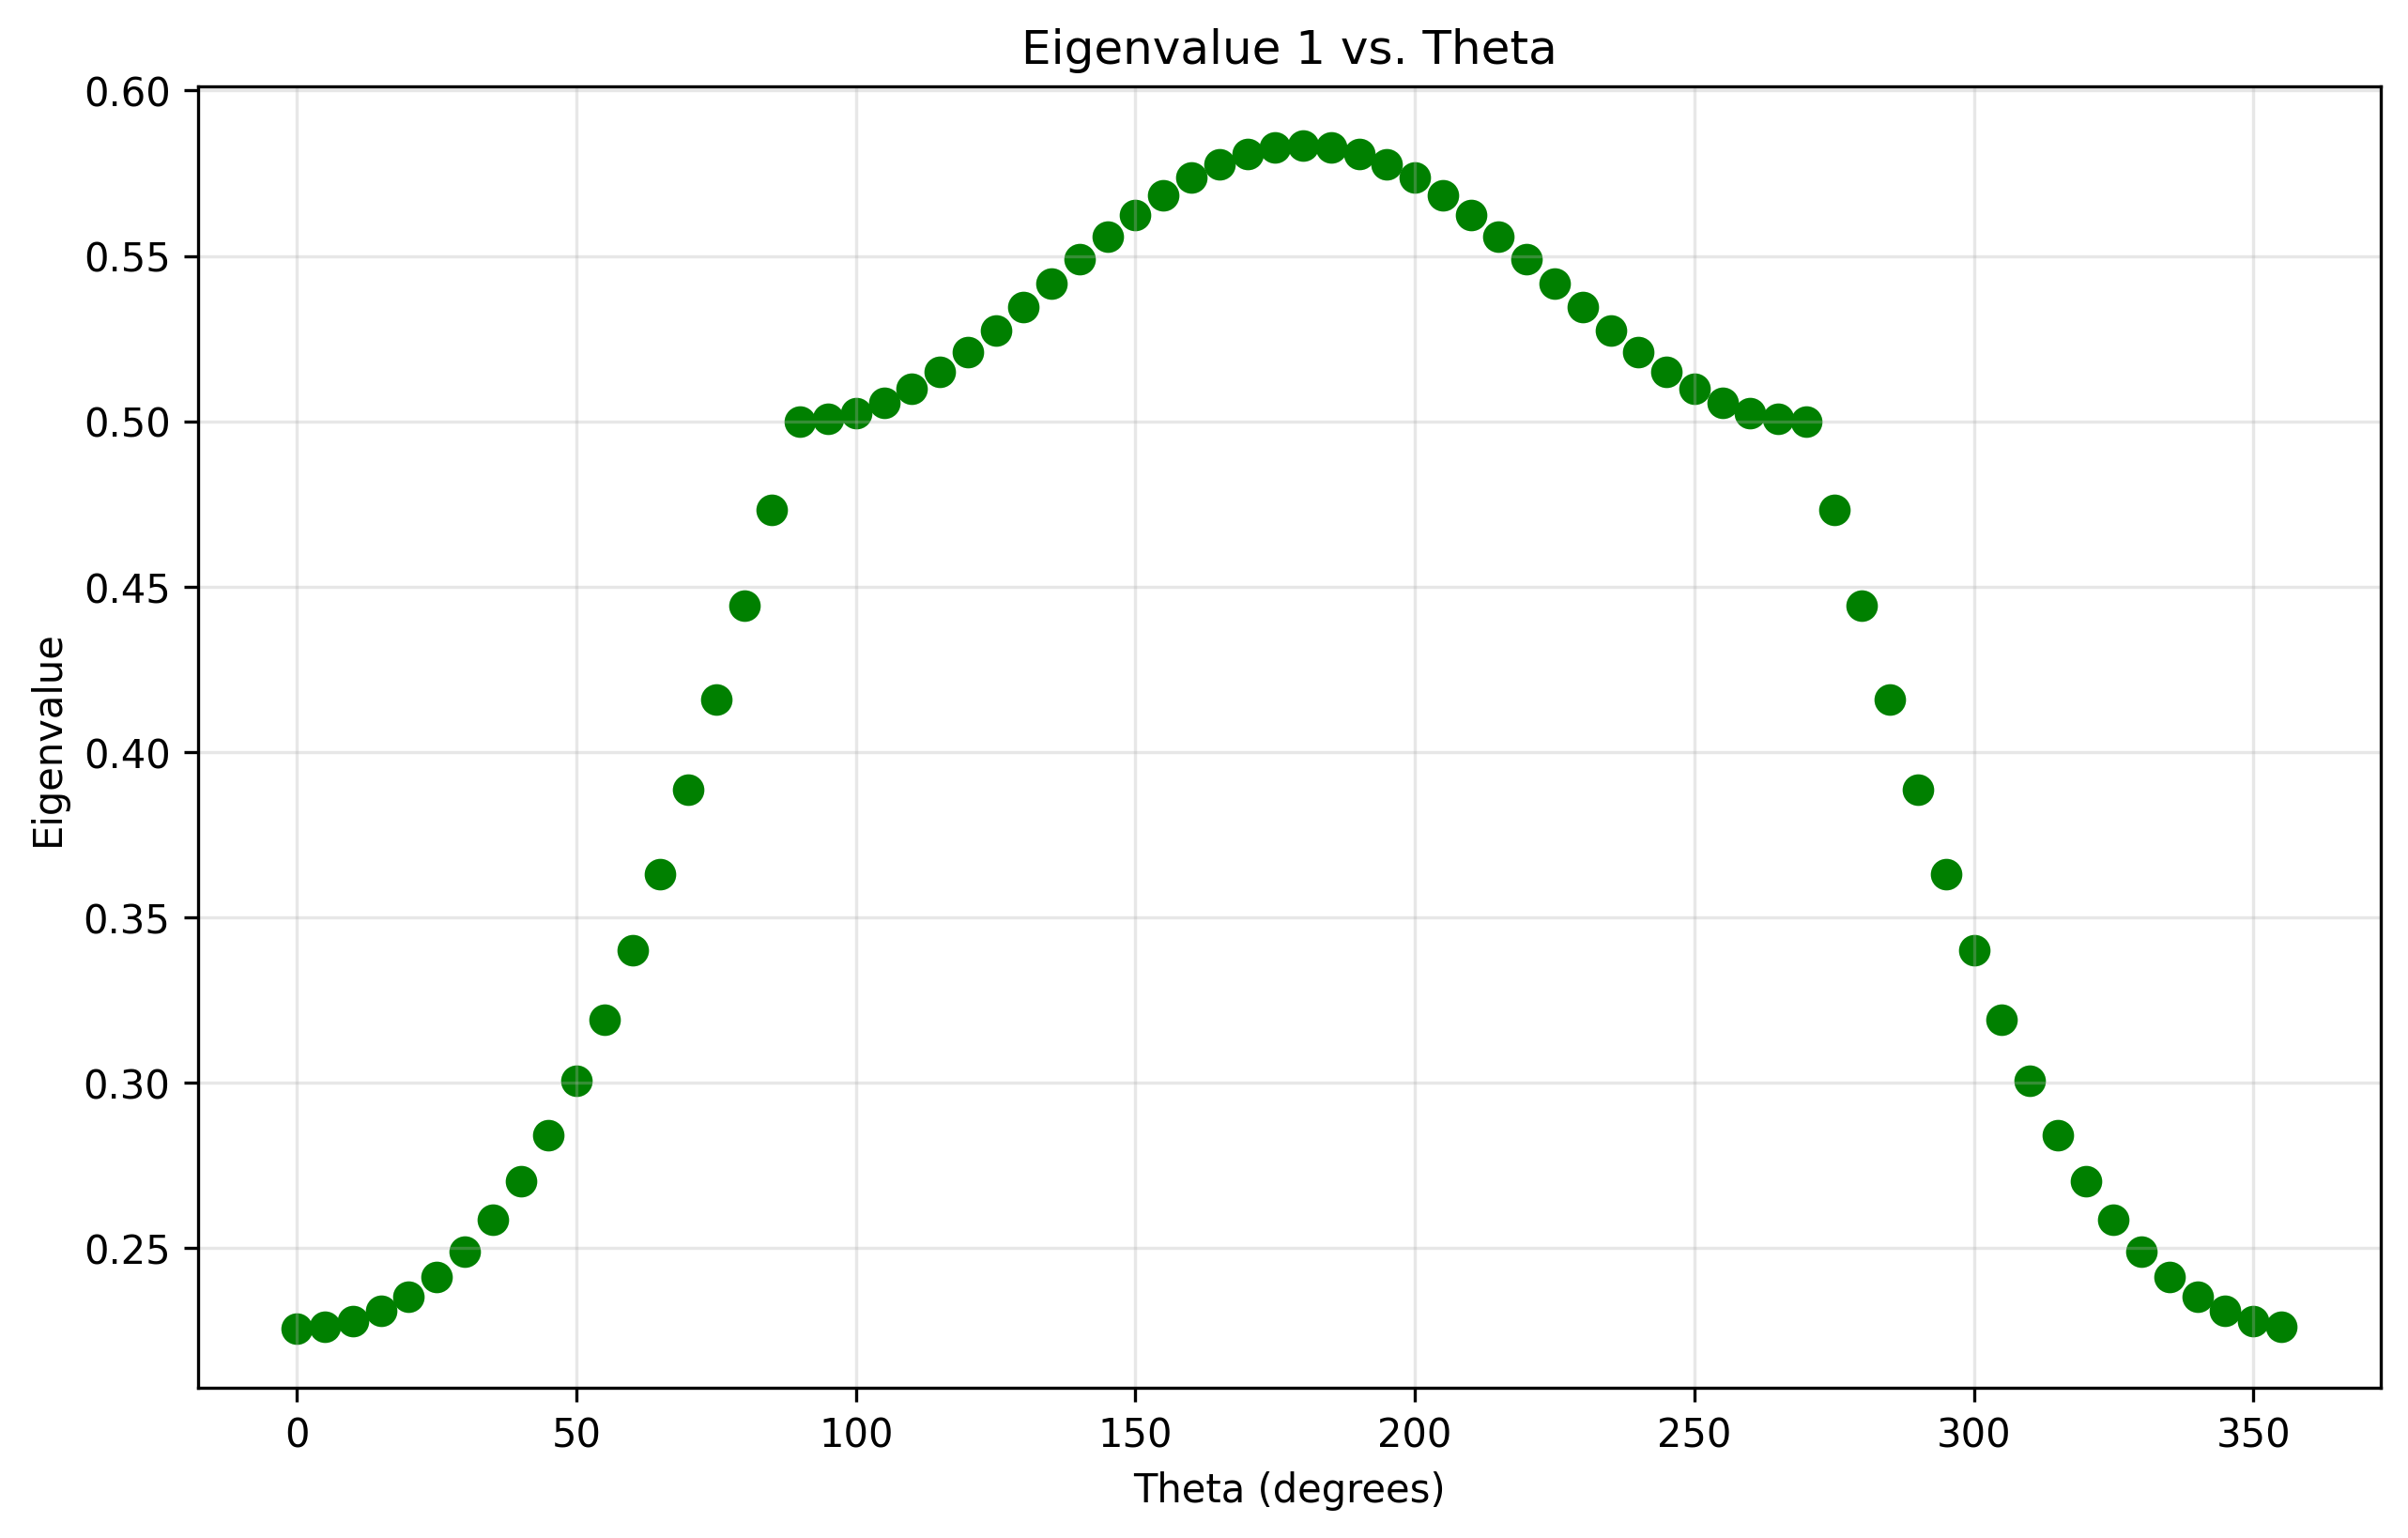
\includegraphics[width=0.8\textwidth]{../example_use/arrowhead_matrix/results/plots/eigenvalue_1_2d.png}
    \caption{Second eigenvalue plotted against $\theta$}
    \label{fig:eigenvalue_1_2d}
\end{figure}

\begin{figure}[H]
    \centering
    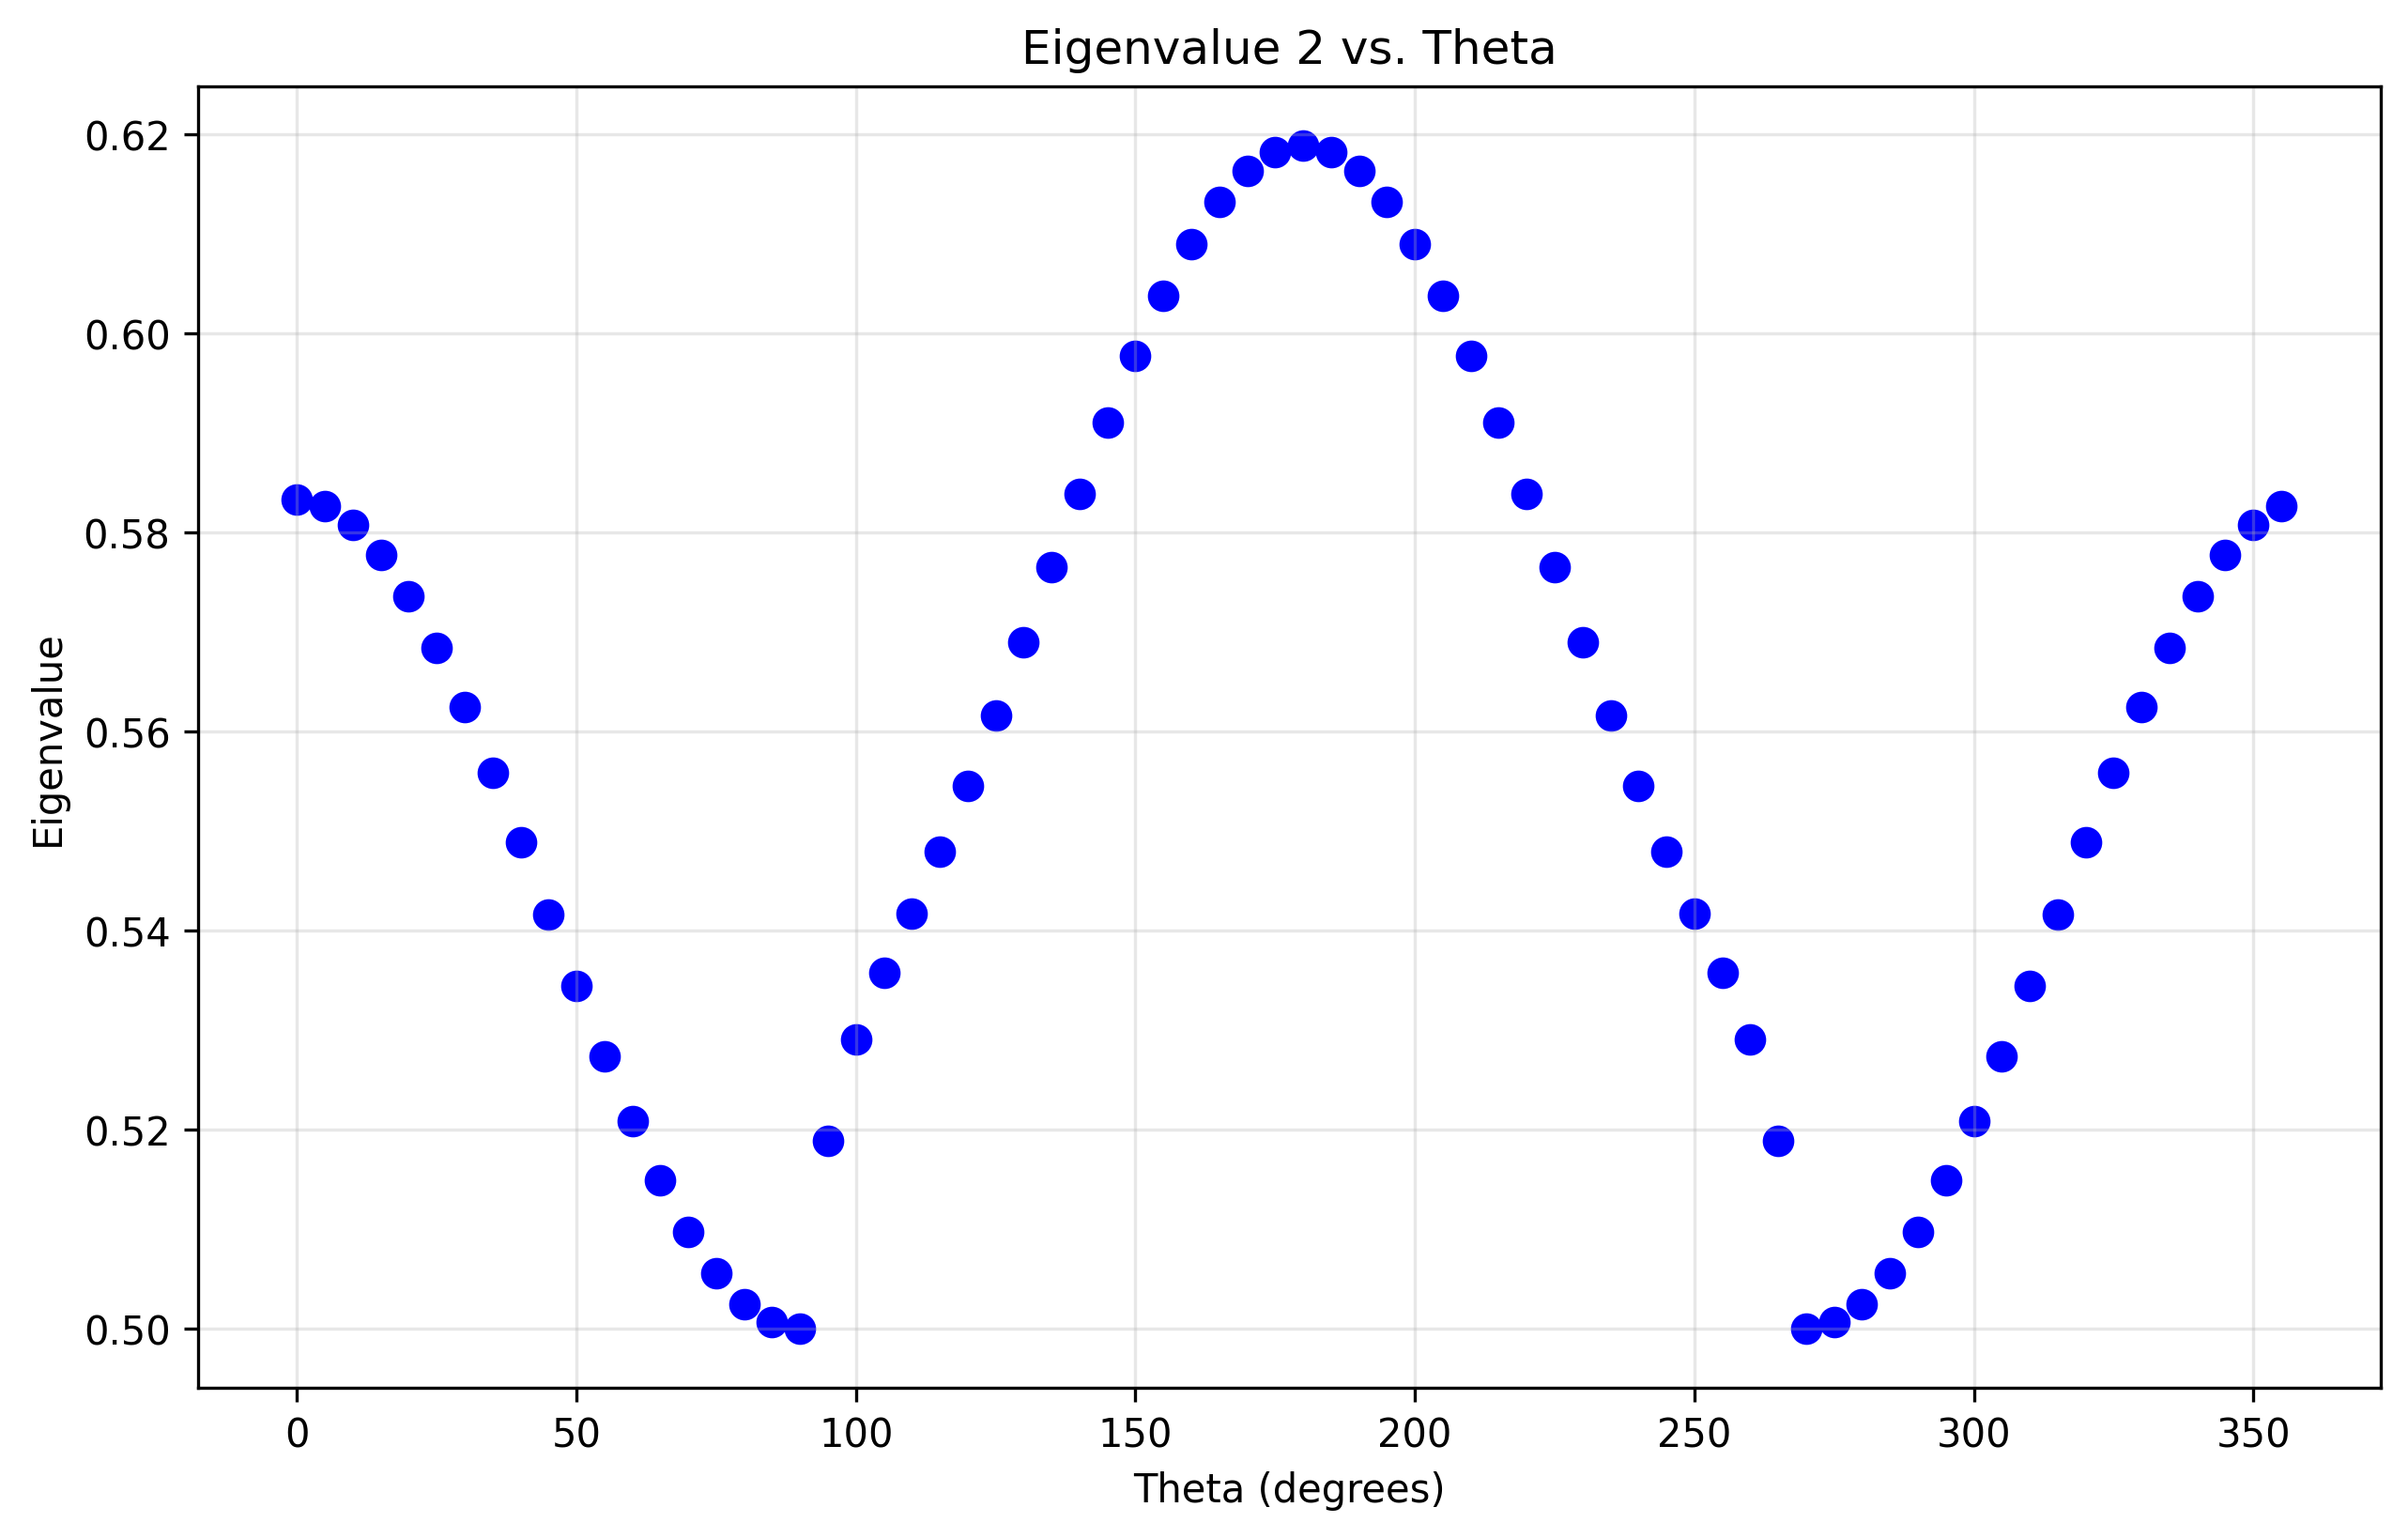
\includegraphics[width=0.8\textwidth]{../example_use/arrowhead_matrix/results/plots/eigenvalue_2_2d.png}
    \caption{Third eigenvalue plotted against $\theta$}
    \label{fig:eigenvalue_2_2d}
\end{figure}

\begin{figure}[H]
    \centering
    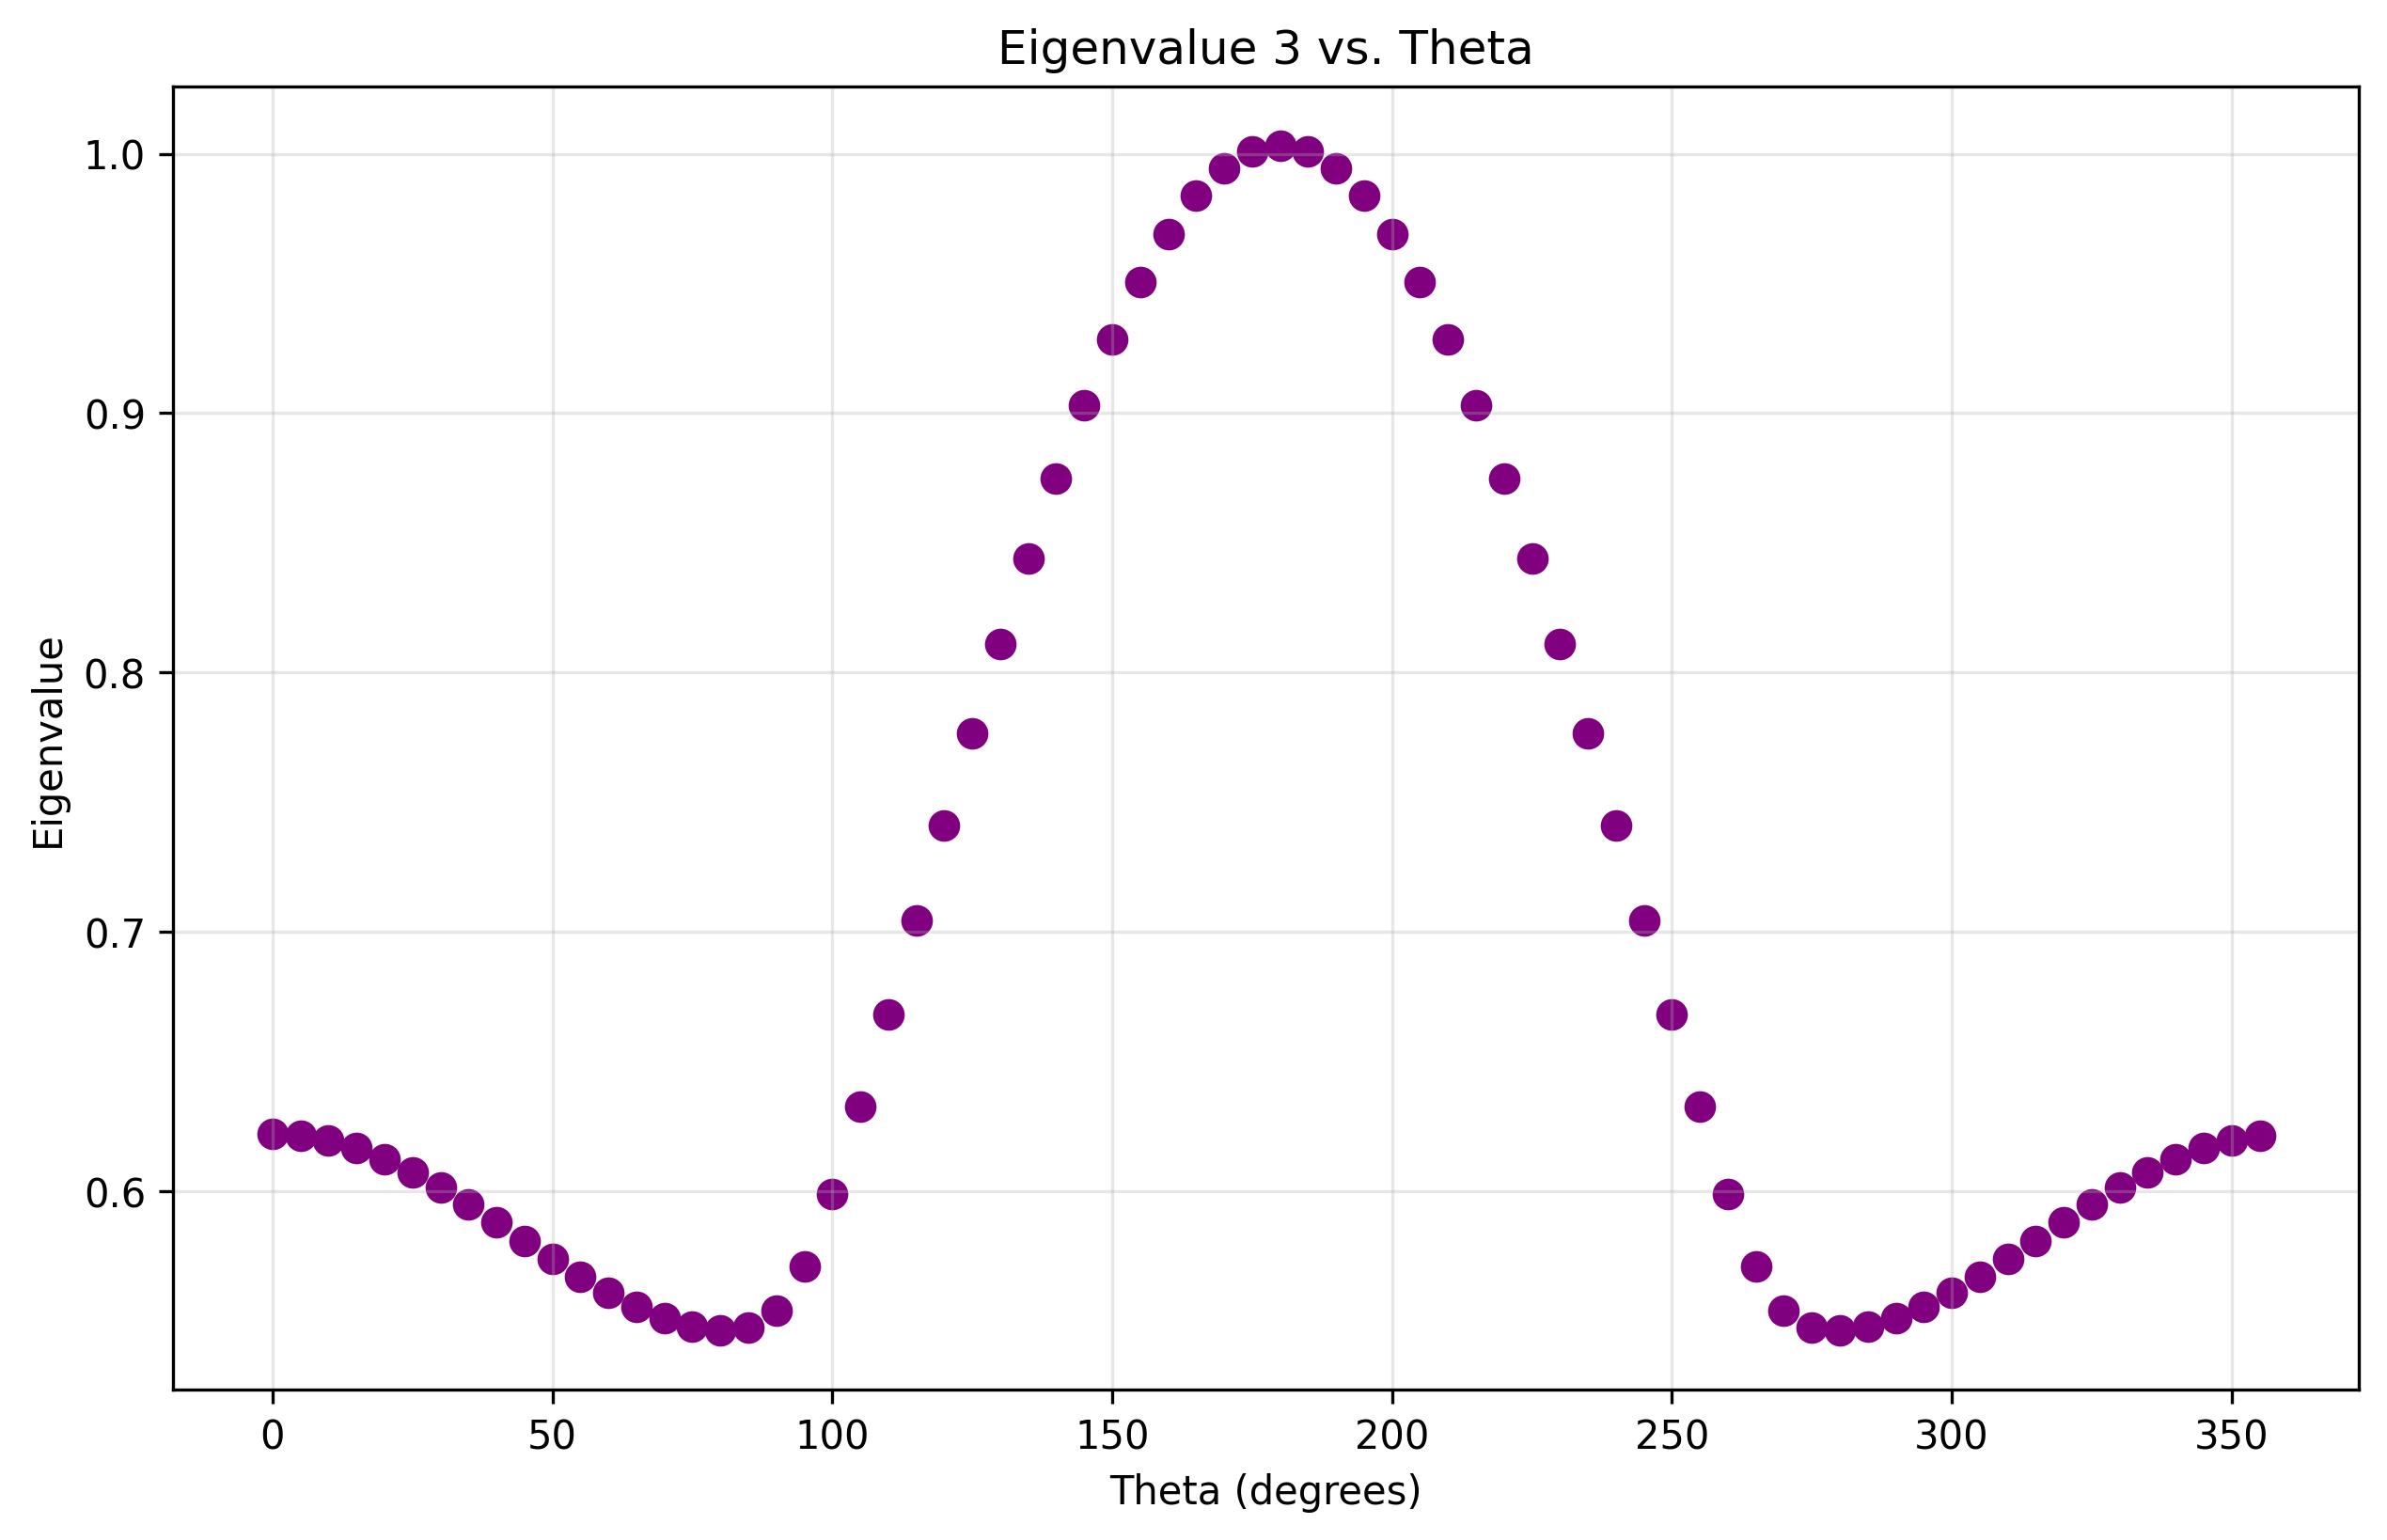
\includegraphics[width=0.8\textwidth]{../example_use/arrowhead_matrix/results/plots/eigenvalue_3_2d.png}
    \caption{Fourth eigenvalue plotted against $\theta$}
    \label{fig:eigenvalue_3_2d}
\end{figure}



\subsection{Eigenvector Visualization}

\subsubsection{Combined Eigenvector Plots}

The eigenvectors of the arrowhead matrices are calculated and visualized in 3D space. Figure \ref{fig:eigenvectors_no_labels} shows the endpoints of all eigenvectors for different values of $\theta$ without labels for clarity.

\begin{figure}[H]
    \centering
    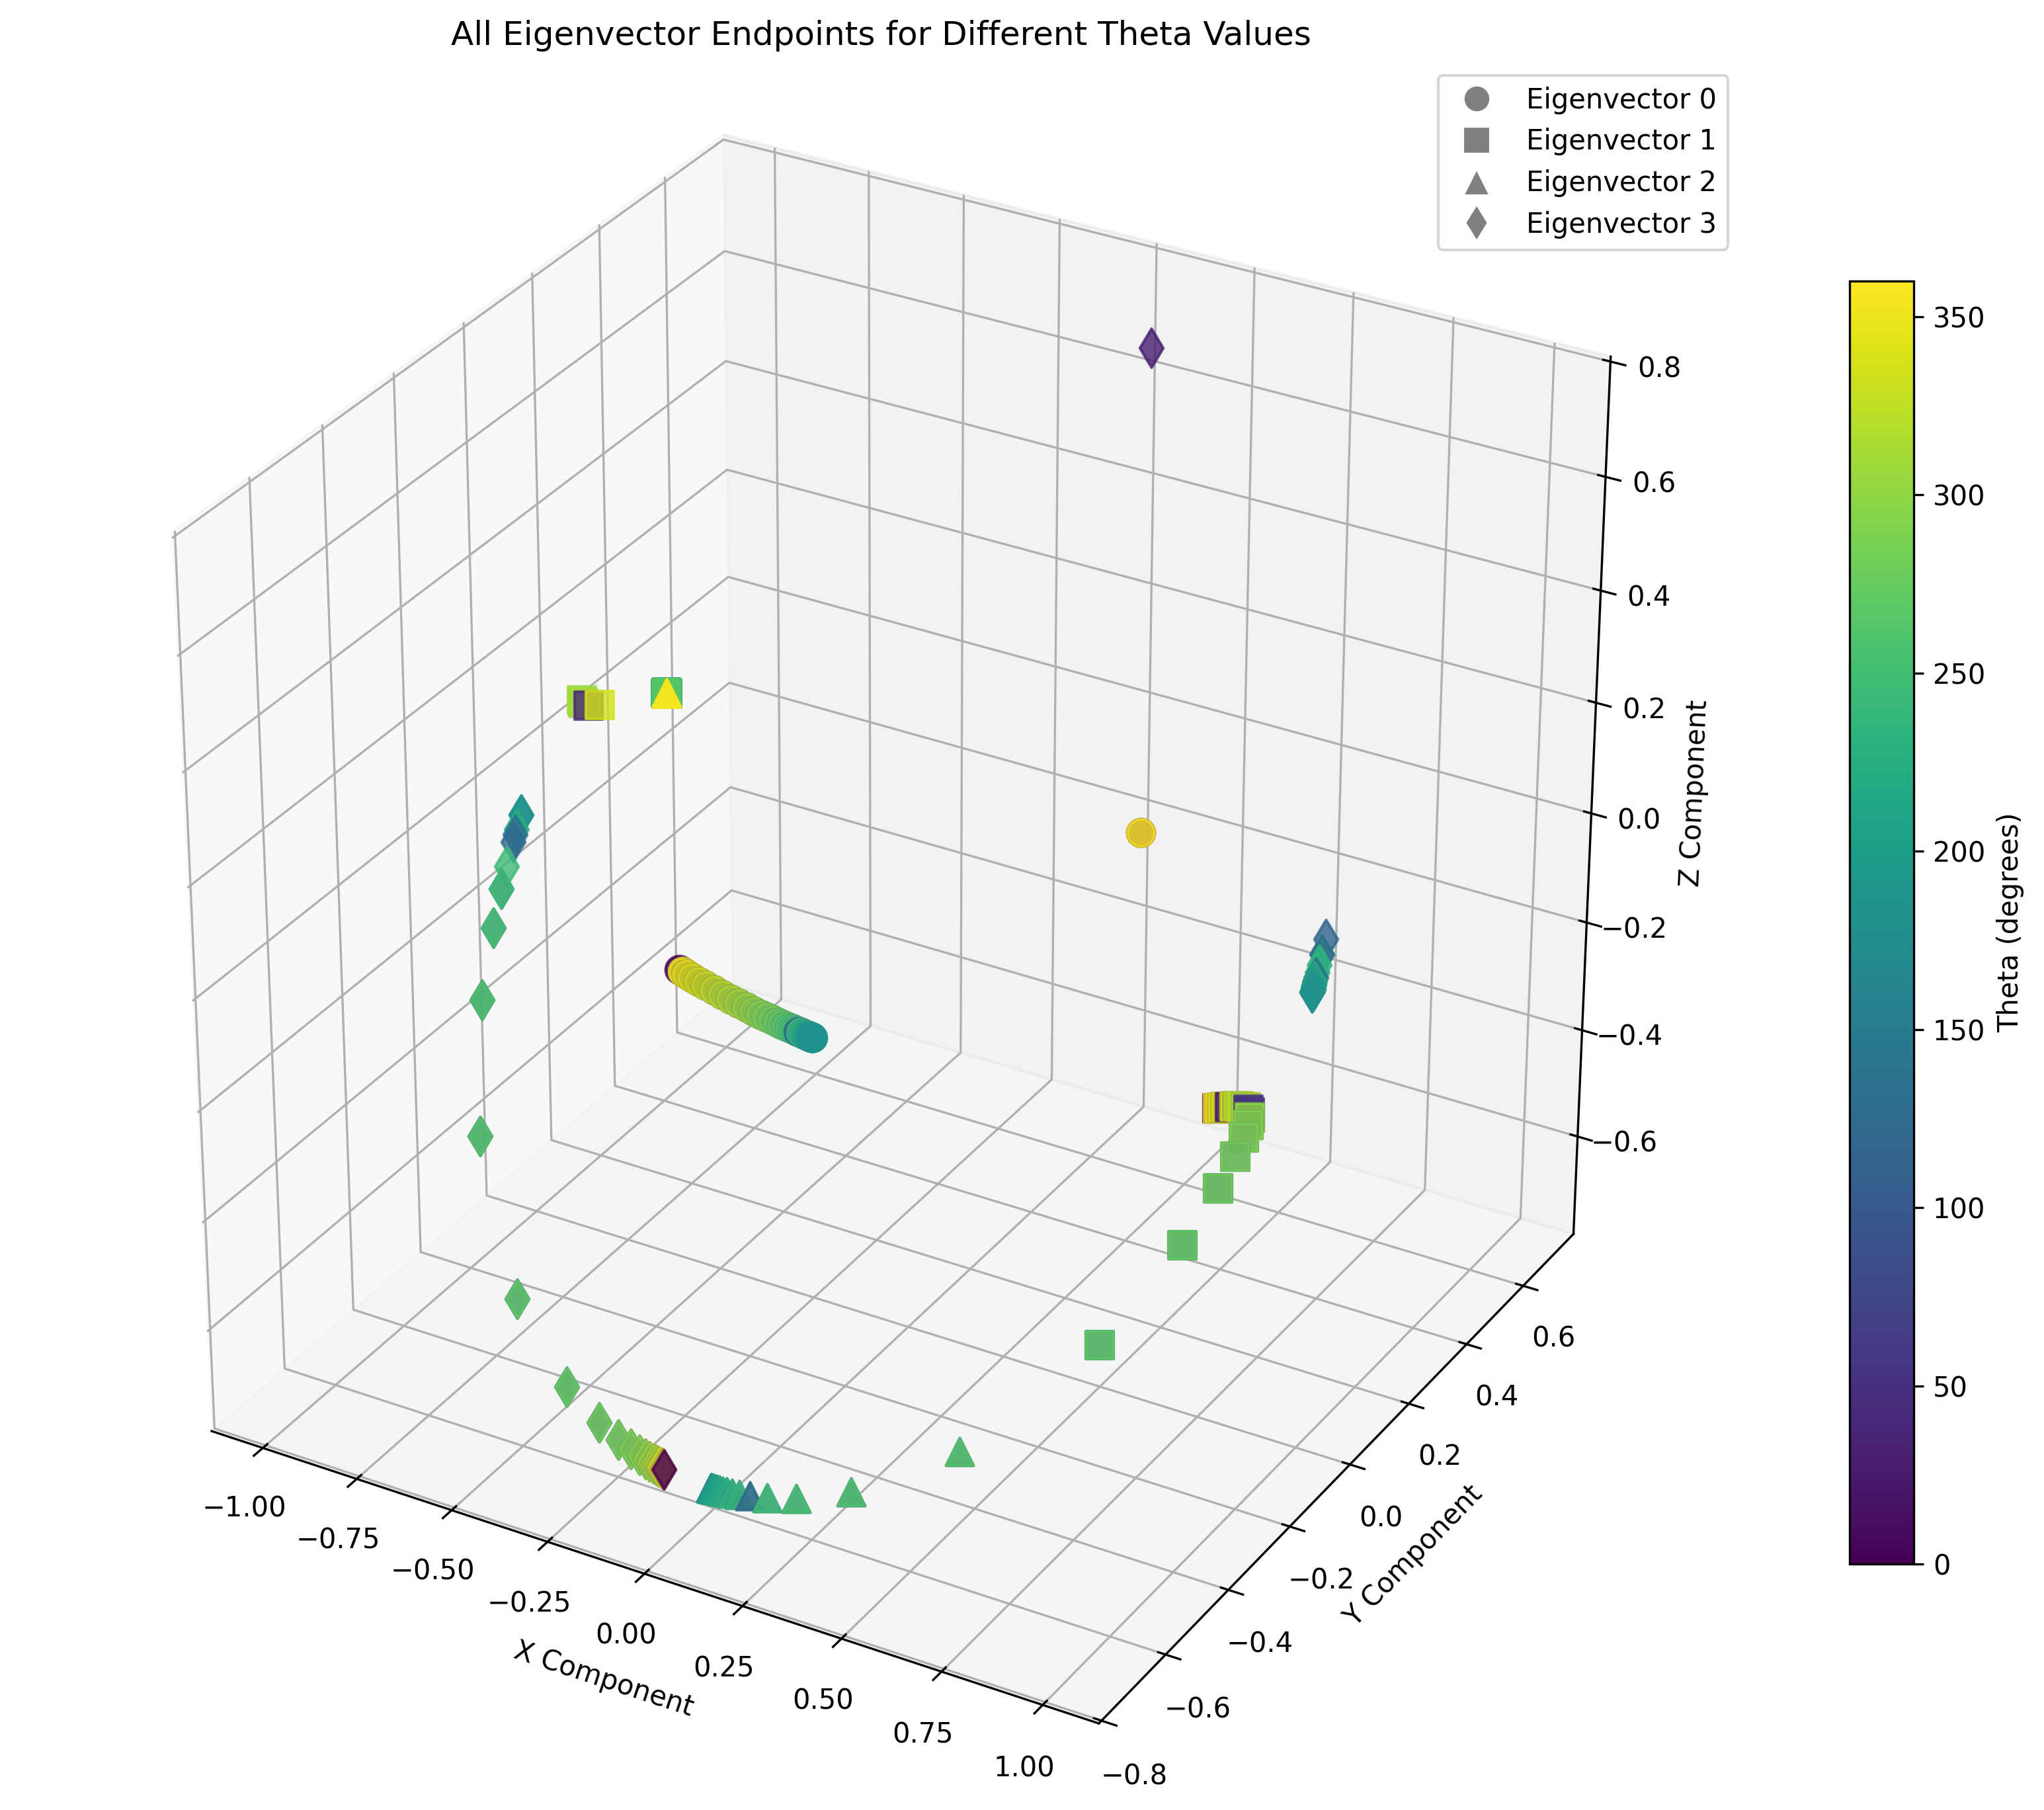
\includegraphics[width=0.8\textwidth]{../example_use/arrowhead_matrix/results/plots/eigenvectors_no_labels.png}
    \caption{3D visualization of all eigenvector endpoints for 72 theta steps (without labels)}
    \label{fig:eigenvectors_no_labels}
\end{figure}



\subsubsection{Individual Eigenvector Plots}

Individual plots for each eigenvector are generated to provide a clearer view of how each eigenvector changes with $\theta$. Figures \ref{fig:eigenvector_0_no_labels} through \ref{fig:eigenvector_3_no_labels} show the plots for each eigenvector without labels.

\begin{figure}[H]
    \centering
    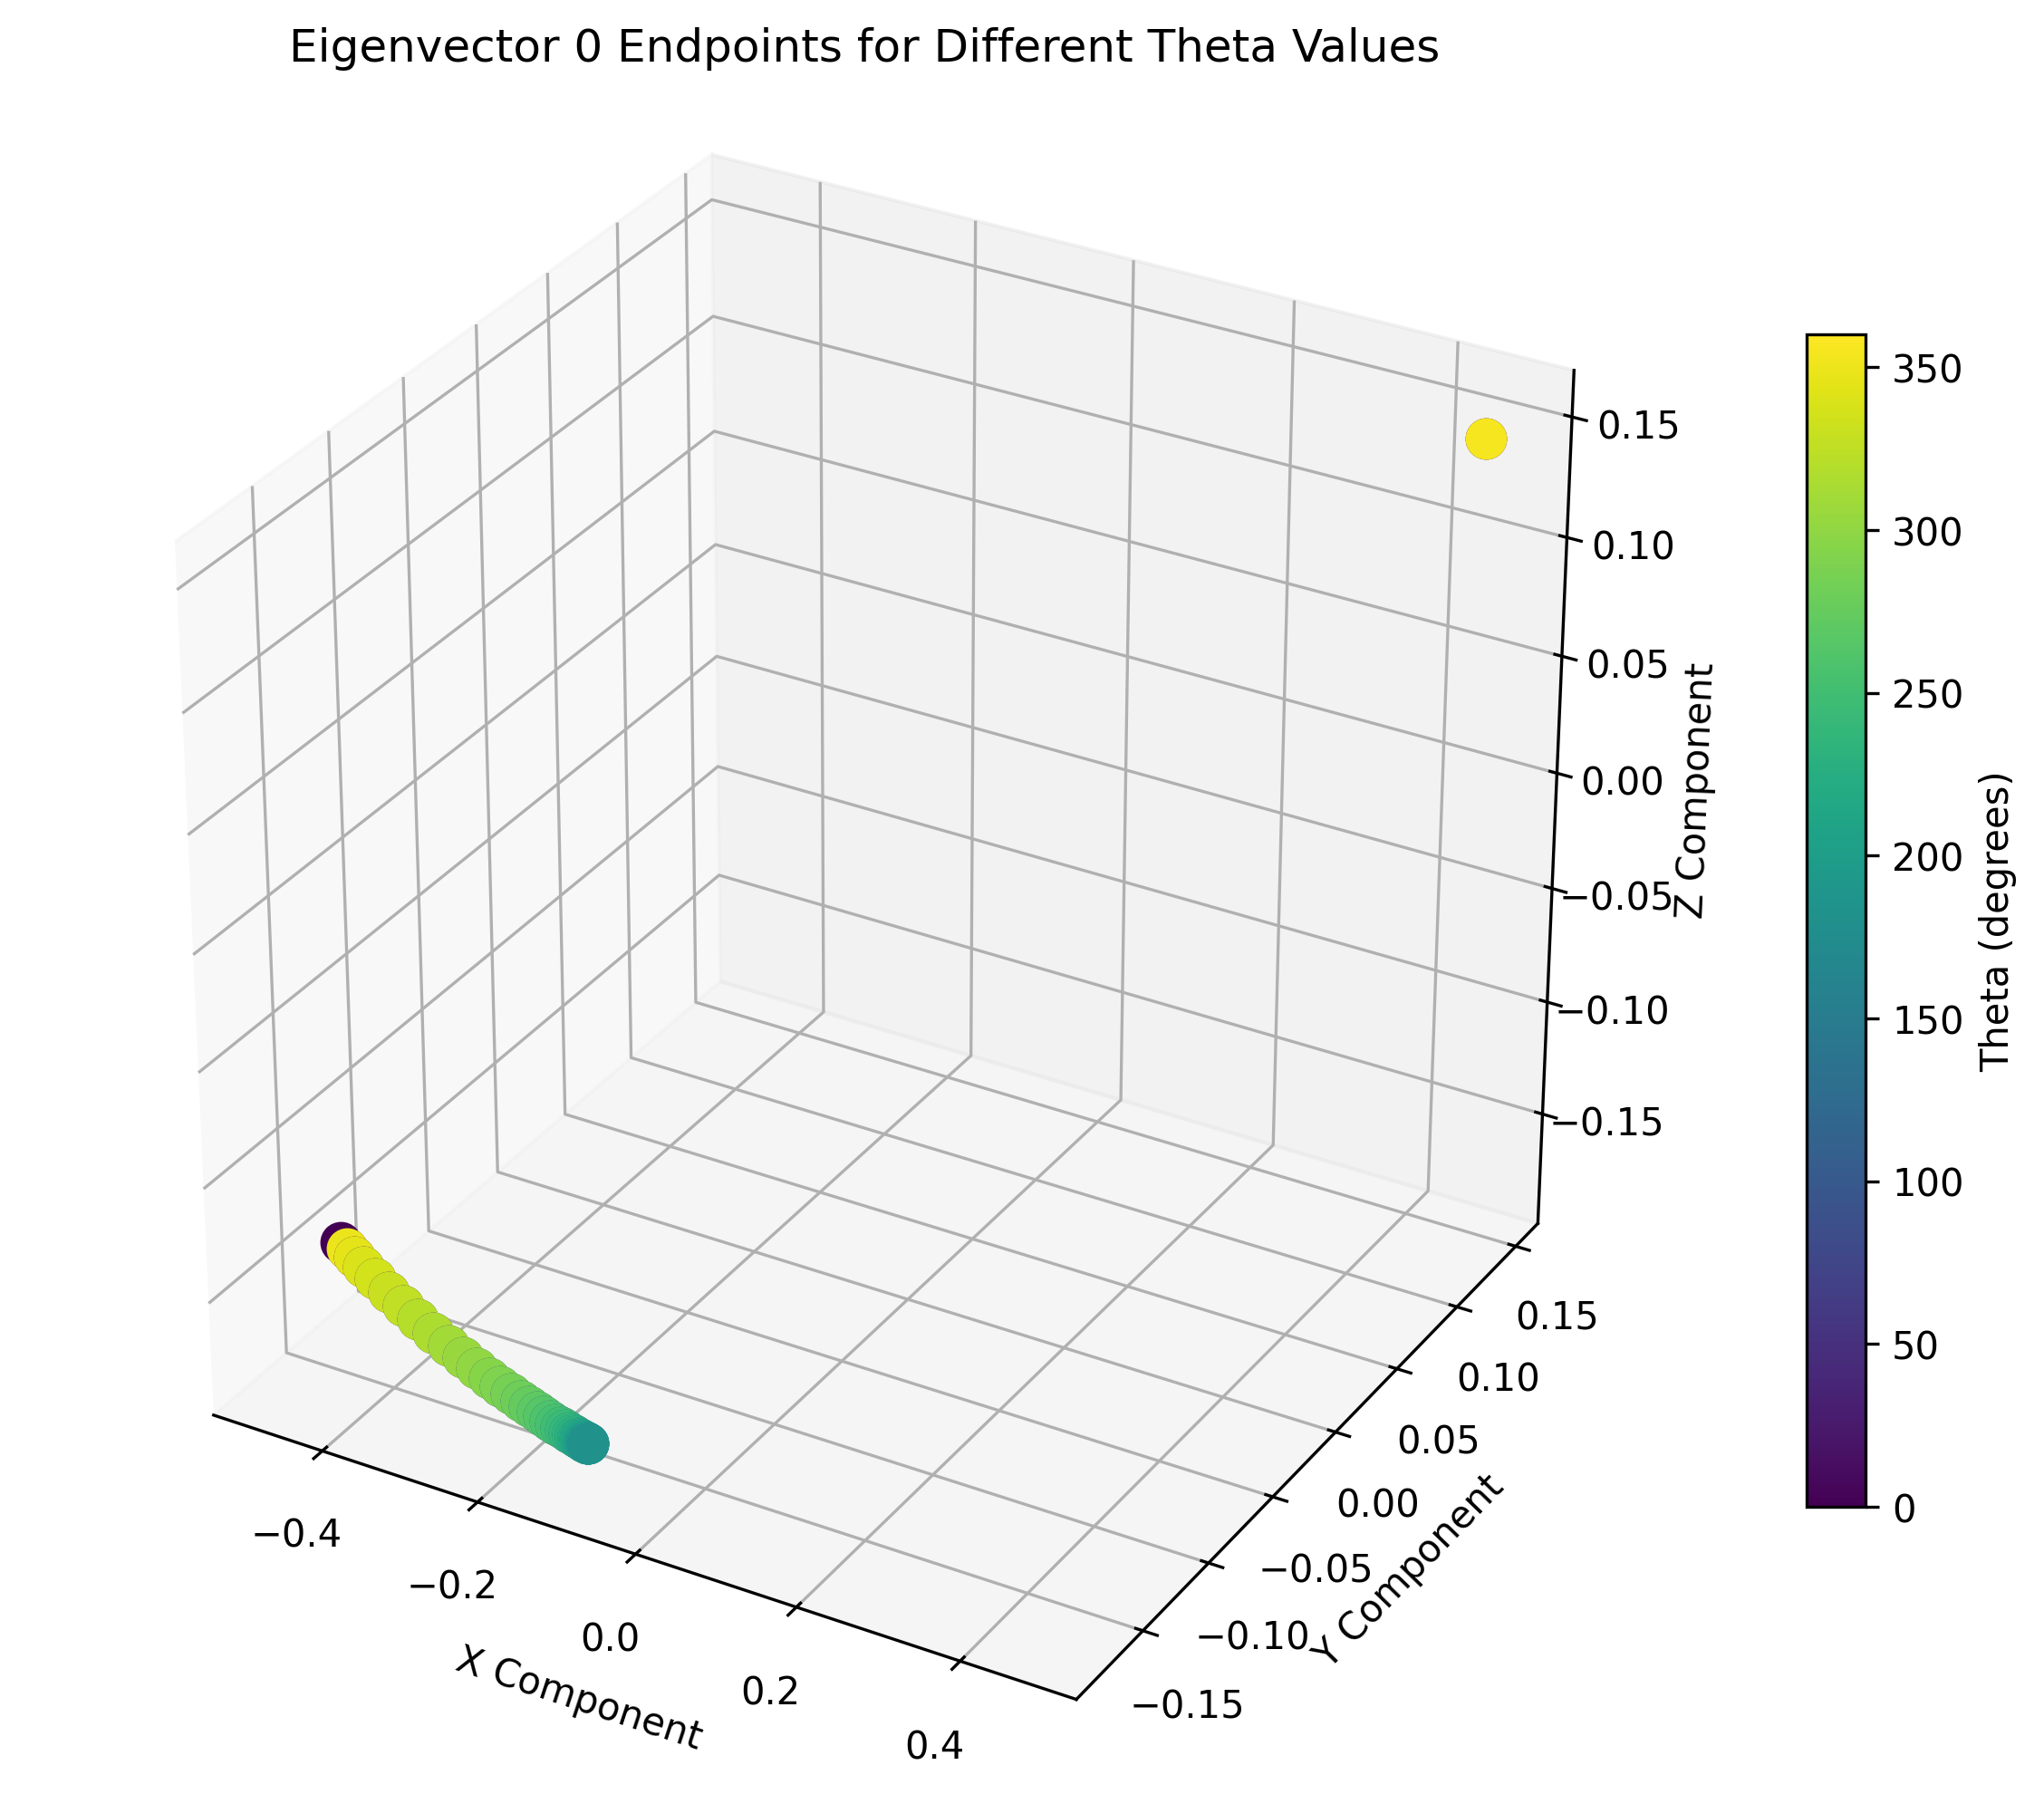
\includegraphics[width=0.8\textwidth]{../example_use/arrowhead_matrix/results/plots/eigenvector_0_no_labels.png}
    \caption{First eigenvector endpoints for 72 different $\theta$ values (0-360° in 5° increments)}
    \label{fig:eigenvector_0_no_labels}
\end{figure}

\begin{figure}[H]
    \centering
    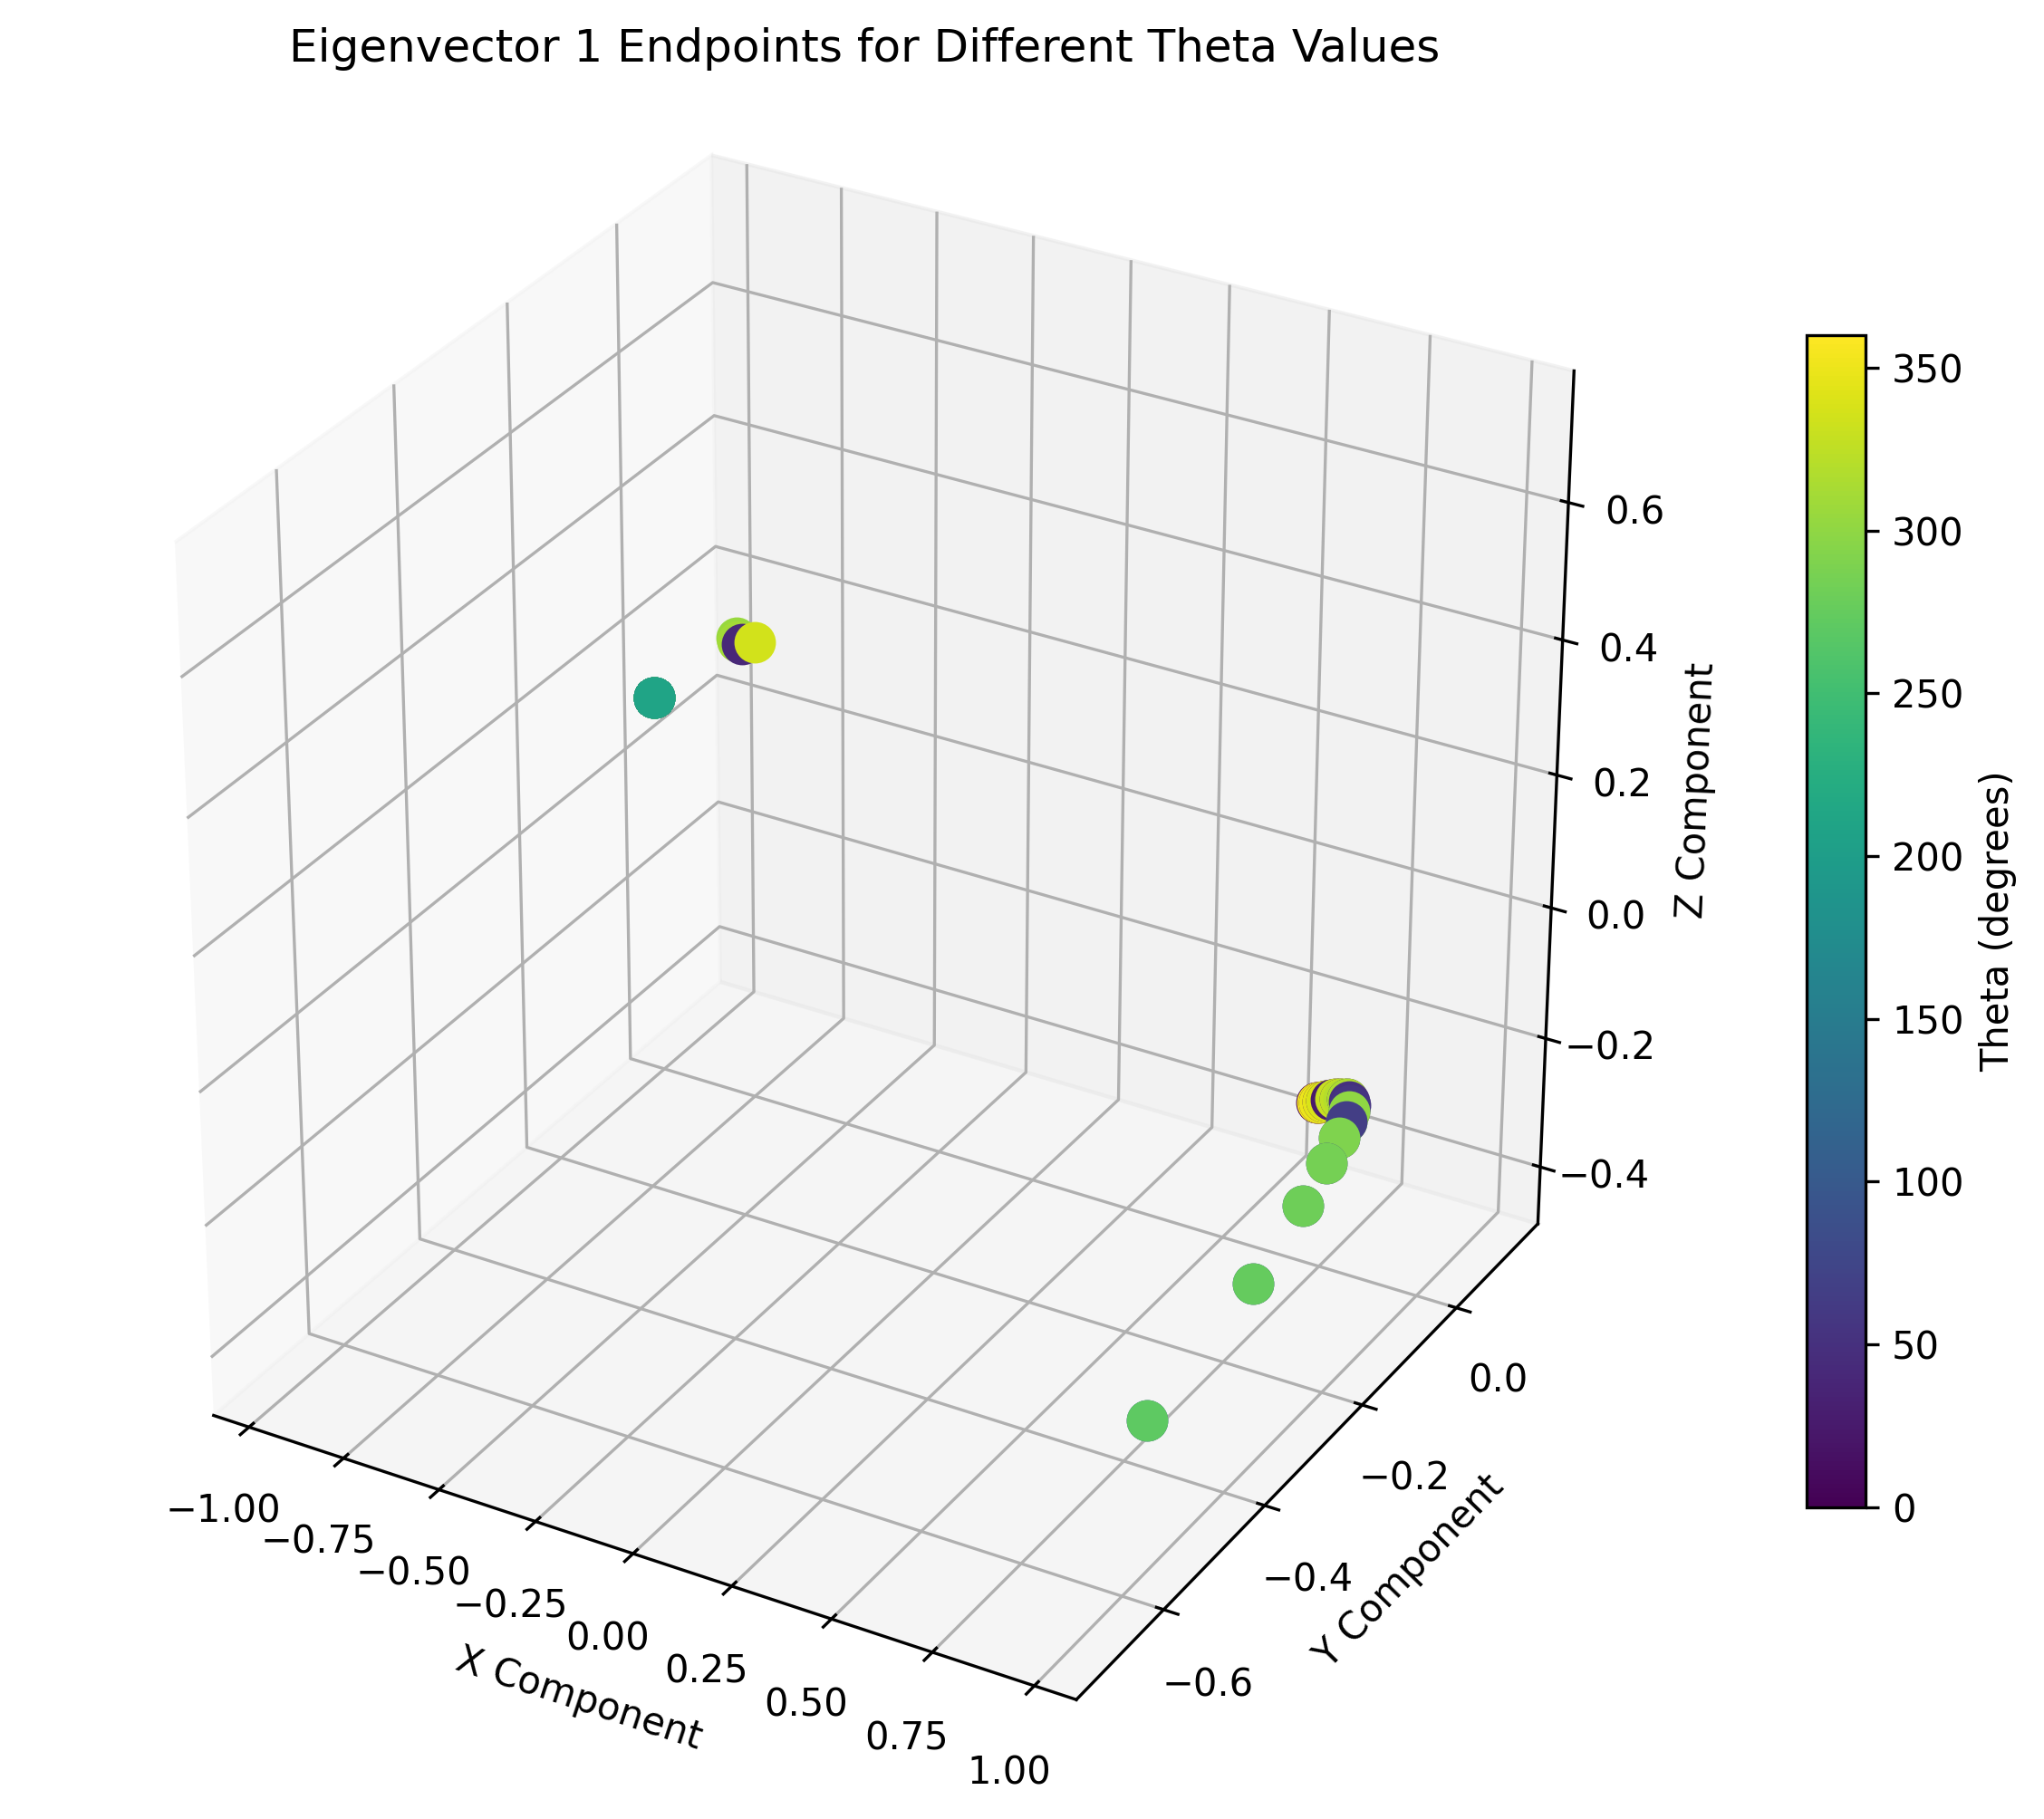
\includegraphics[width=0.8\textwidth]{../example_use/arrowhead_matrix/results/plots/eigenvector_1_no_labels.png}
    \caption{Second eigenvector endpoints for 72 different $\theta$ values (0-360° in 5° increments)}
    \label{fig:eigenvector_1_no_labels}
\end{figure}

\begin{figure}[H]
    \centering
    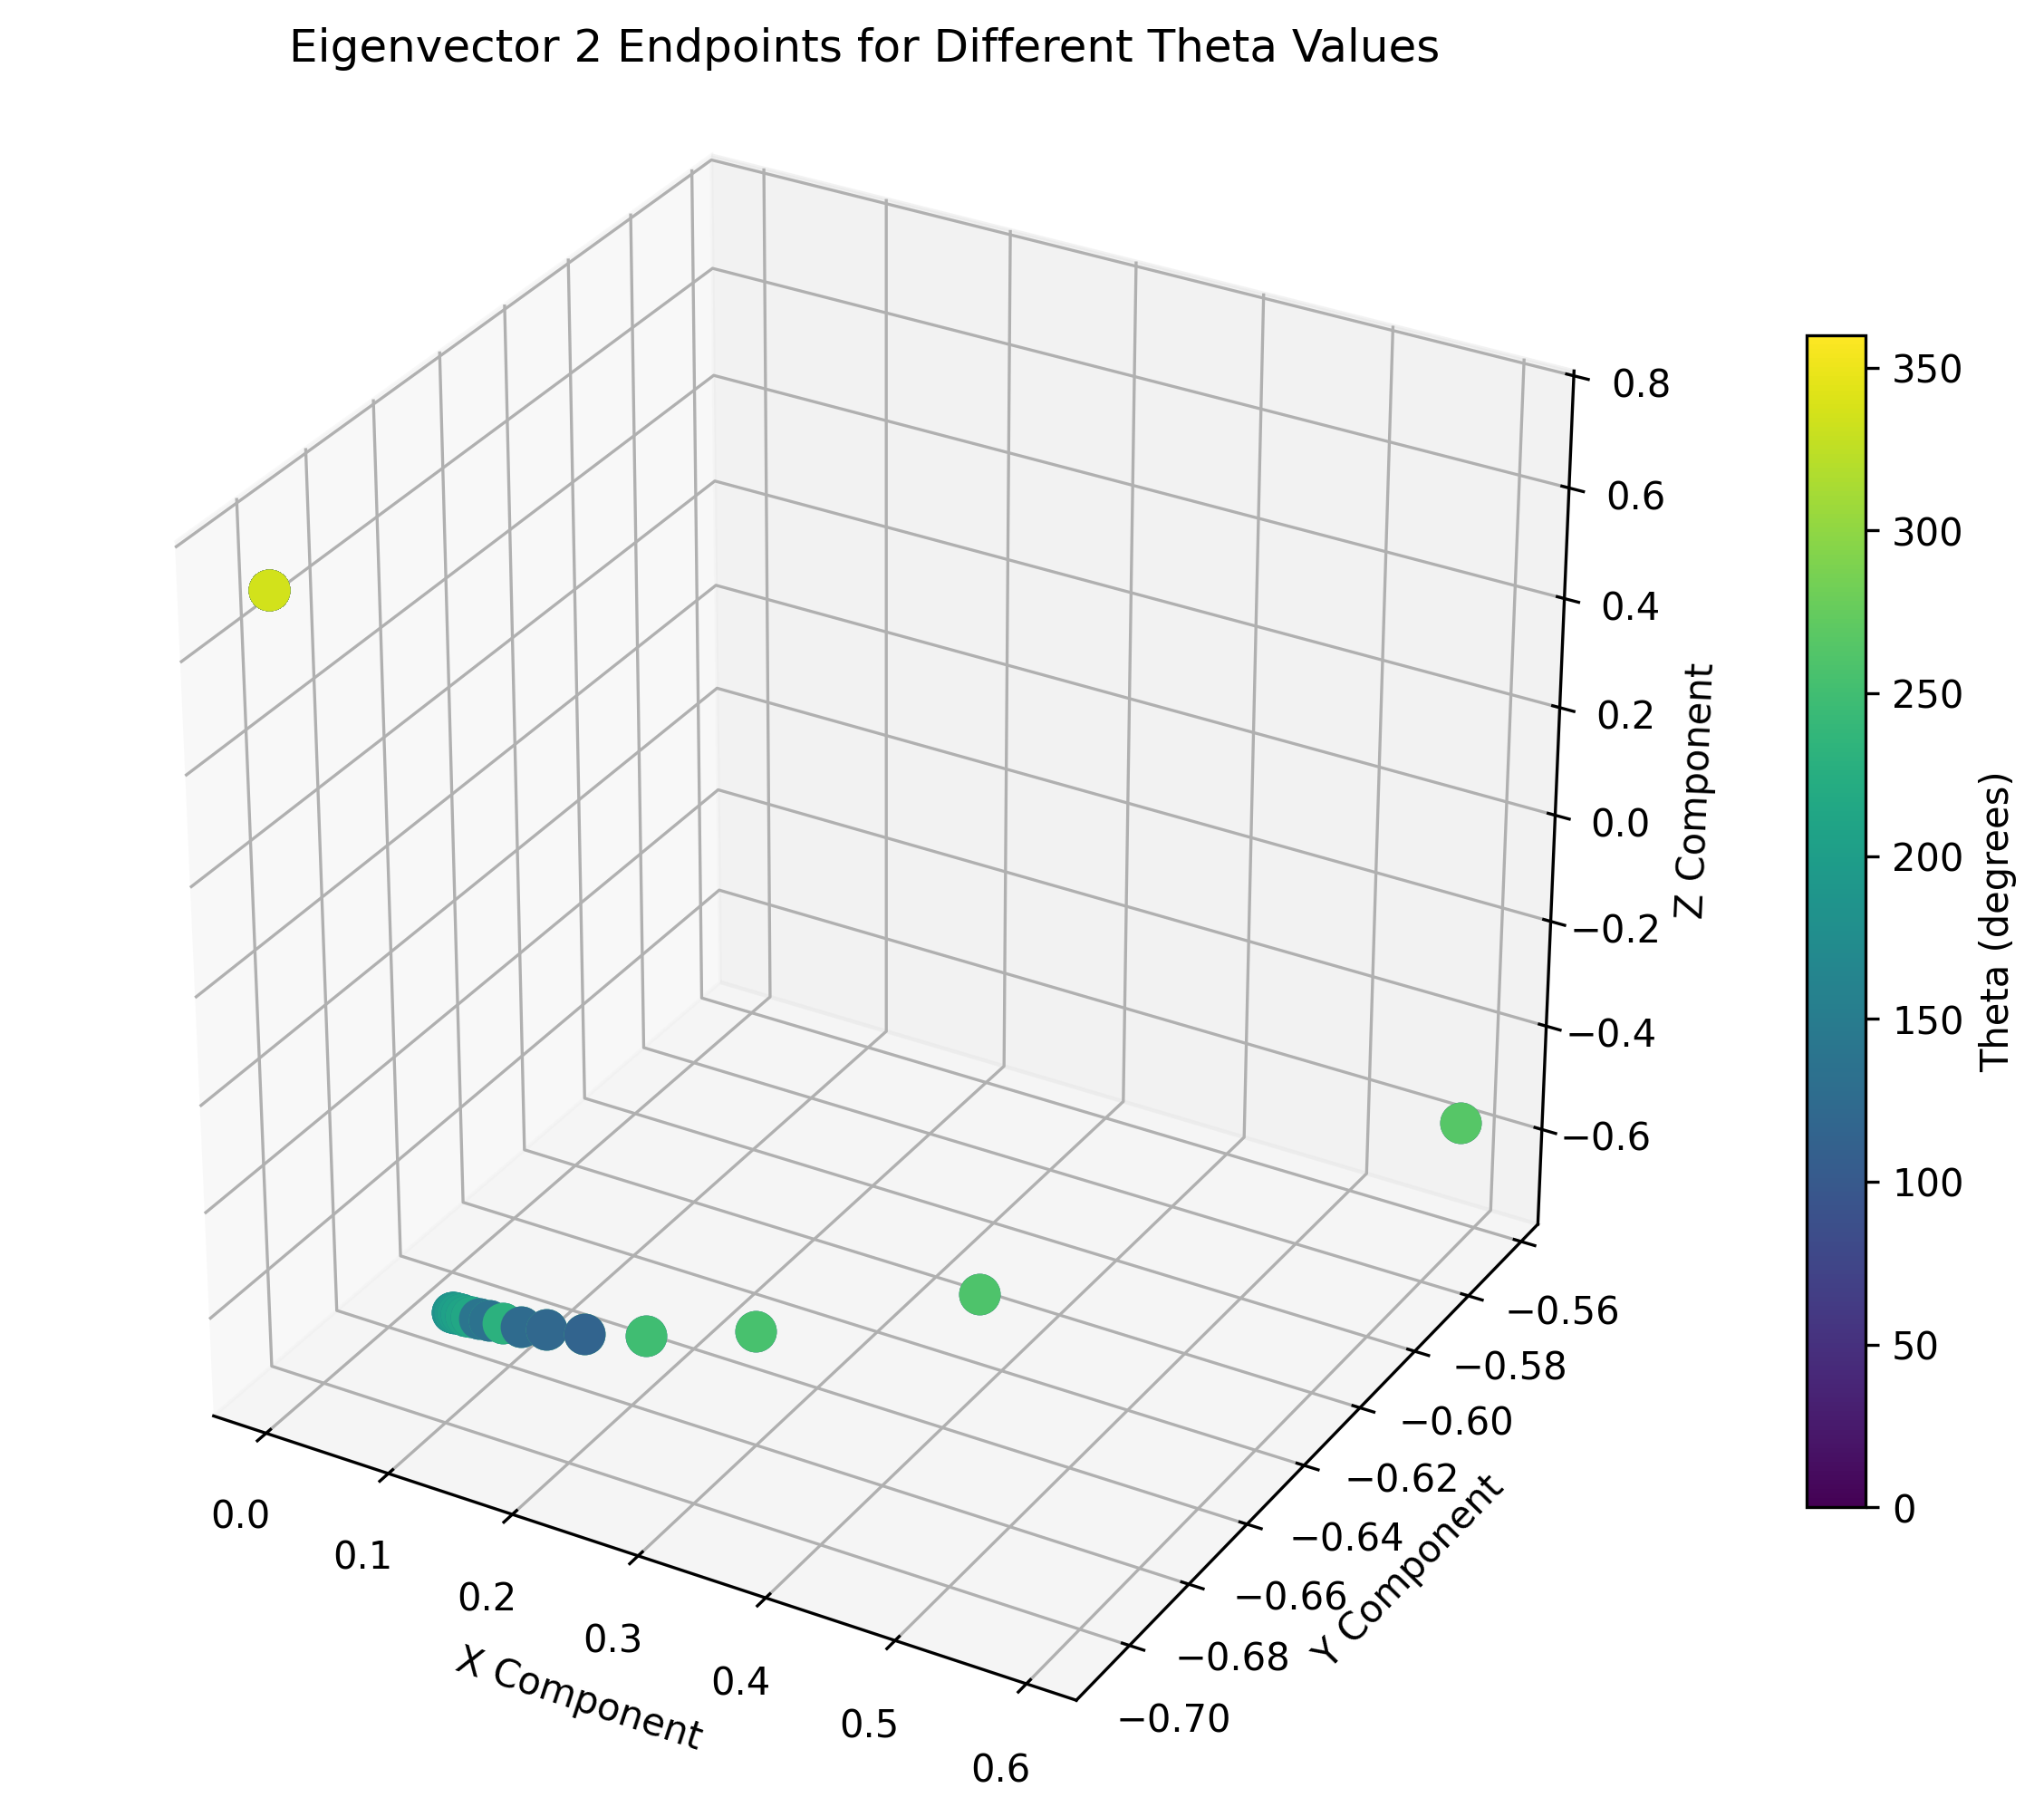
\includegraphics[width=0.8\textwidth]{../example_use/arrowhead_matrix/results/plots/eigenvector_2_no_labels.png}
    \caption{Third eigenvector endpoints for 72 different $\theta$ values (0-360° in 5° increments)}
    \label{fig:eigenvector_2_no_labels}
\end{figure}

\begin{figure}[H]
    \centering
    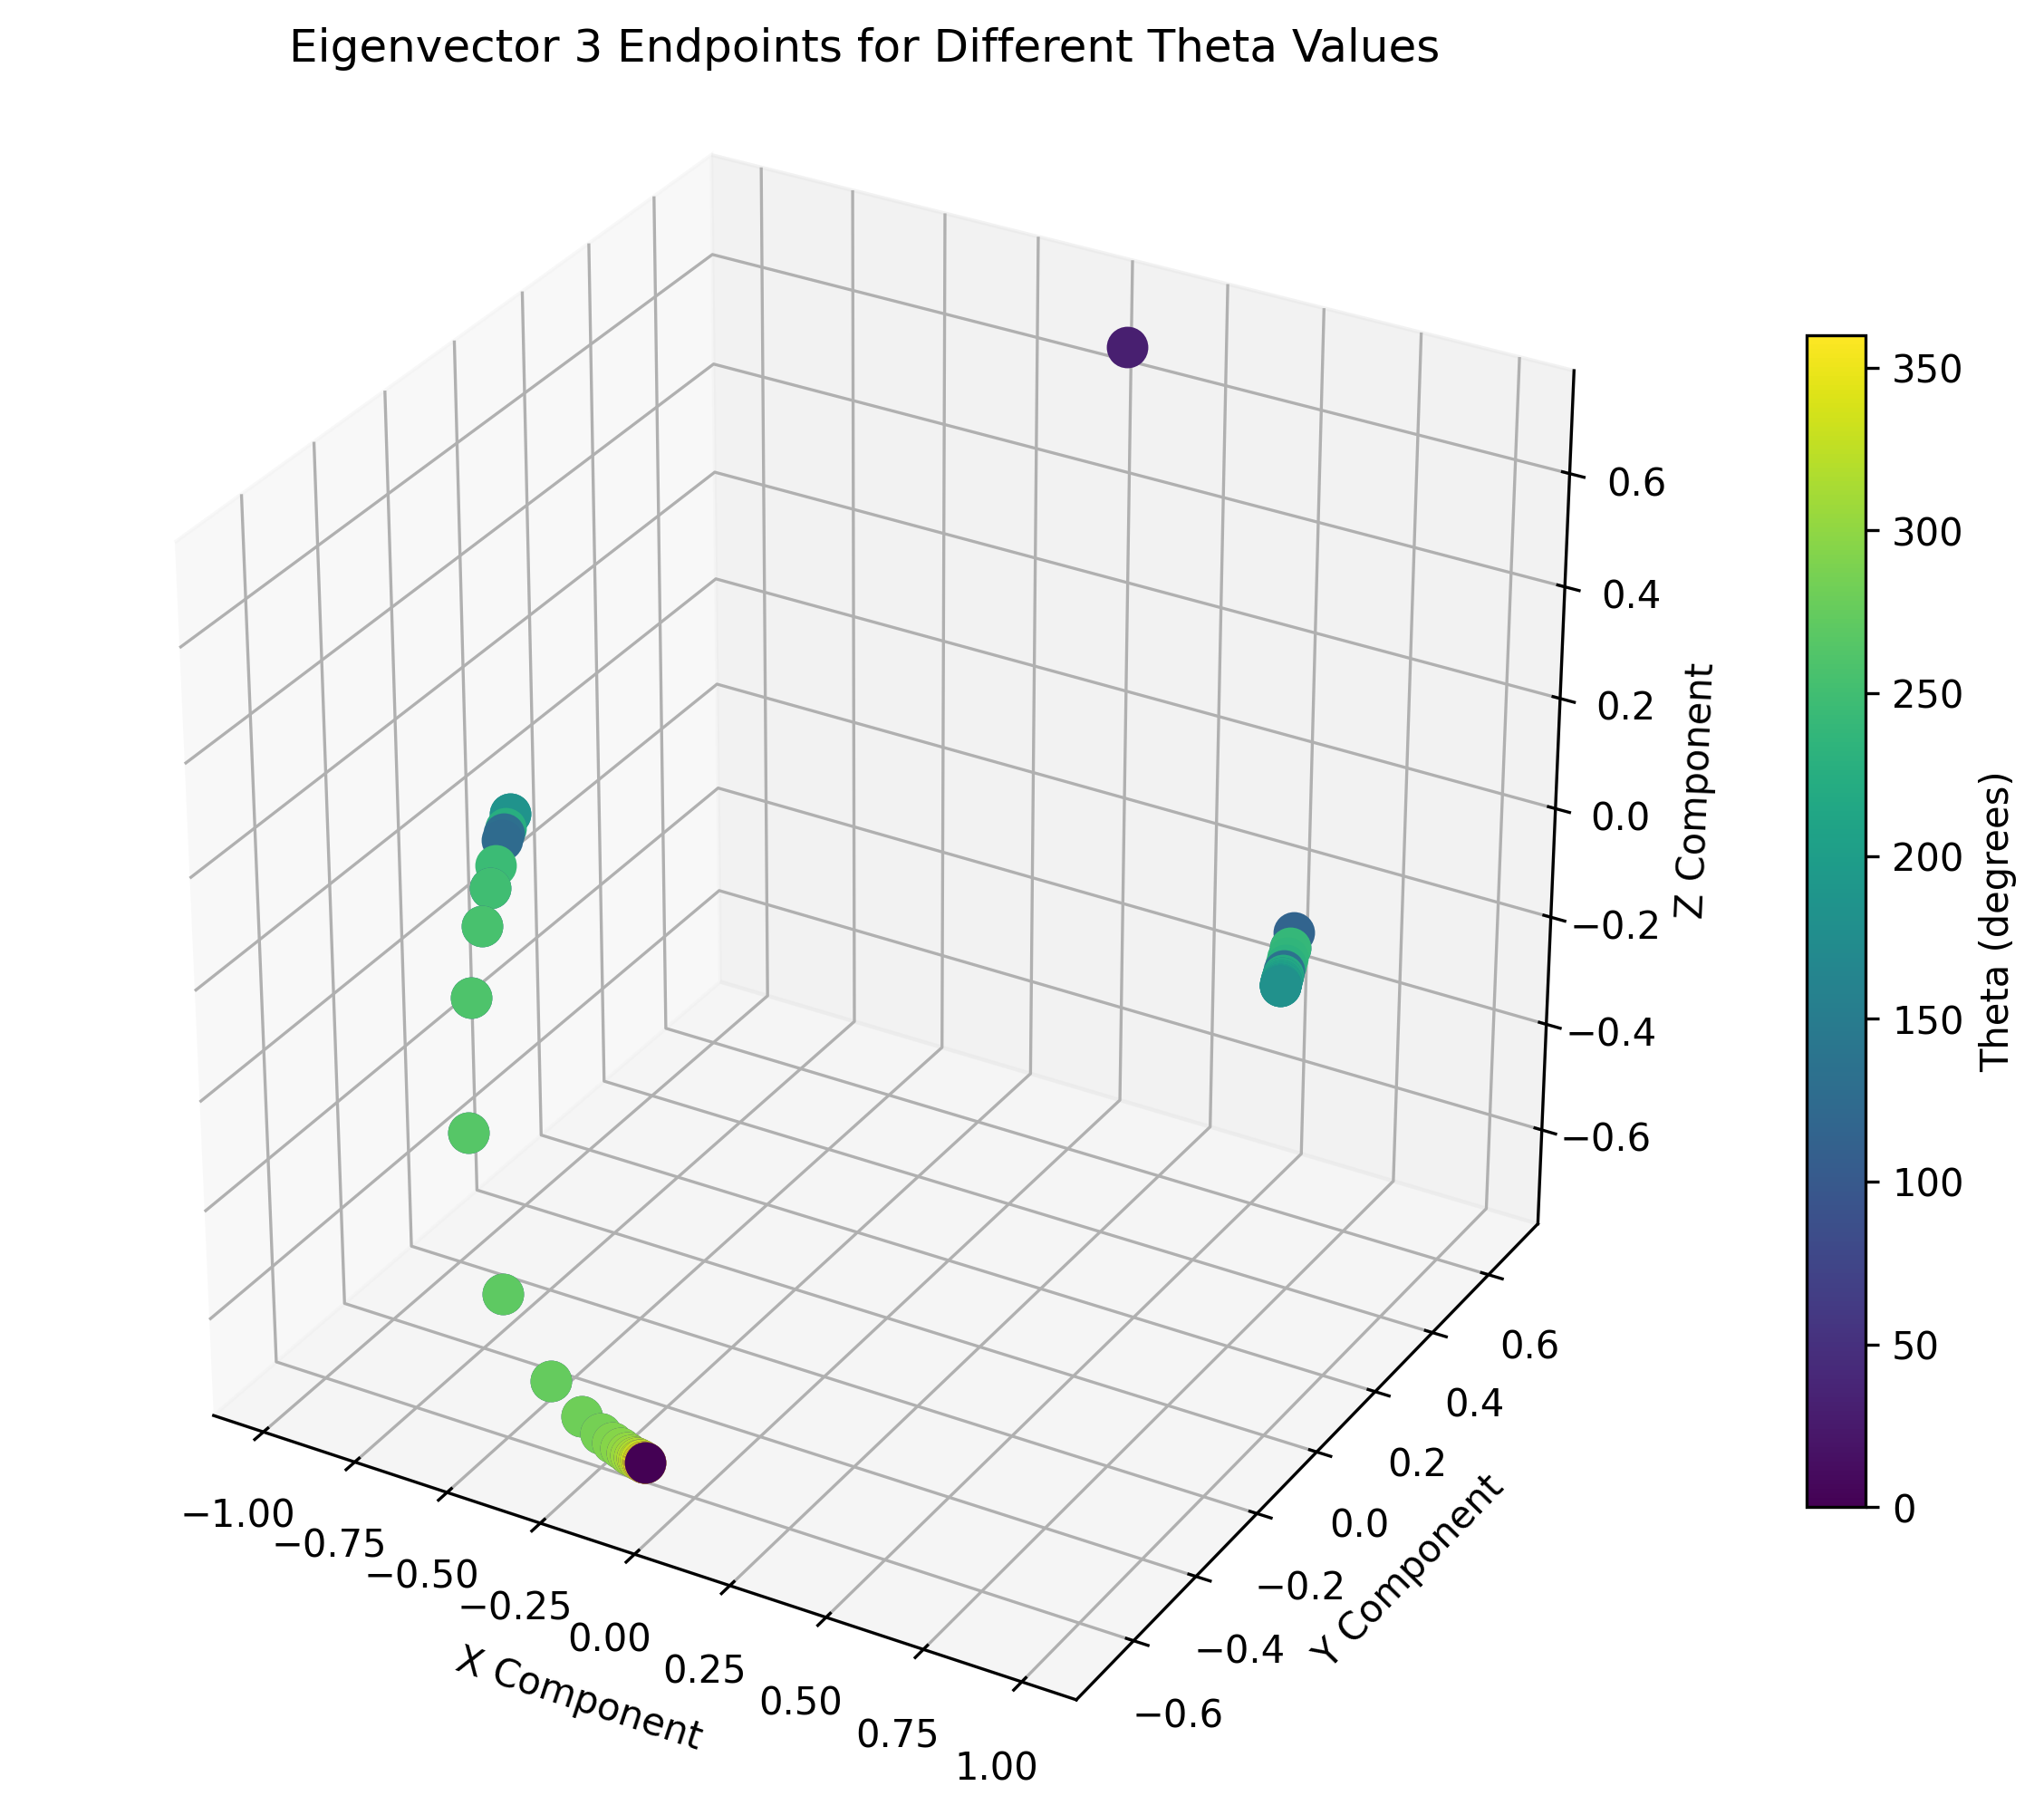
\includegraphics[width=0.8\textwidth]{../example_use/arrowhead_matrix/results/plots/eigenvector_3_no_labels.png}
    \caption{Fourth eigenvector endpoints for 72 different $\theta$ values (0-360° in 5° increments)}
    \label{fig:eigenvector_3_no_labels}
\end{figure}

\subsection{R Vectors Visualization}

The R vectors used to generate the arrowhead matrices are also visualized in 3D space. These vectors form a perfect circle in the plane orthogonal to the x=y=z line. Figure \ref{fig:r_vectors_3d} shows the R vectors for different values of $\theta$.

\begin{figure}[H]
    \centering
    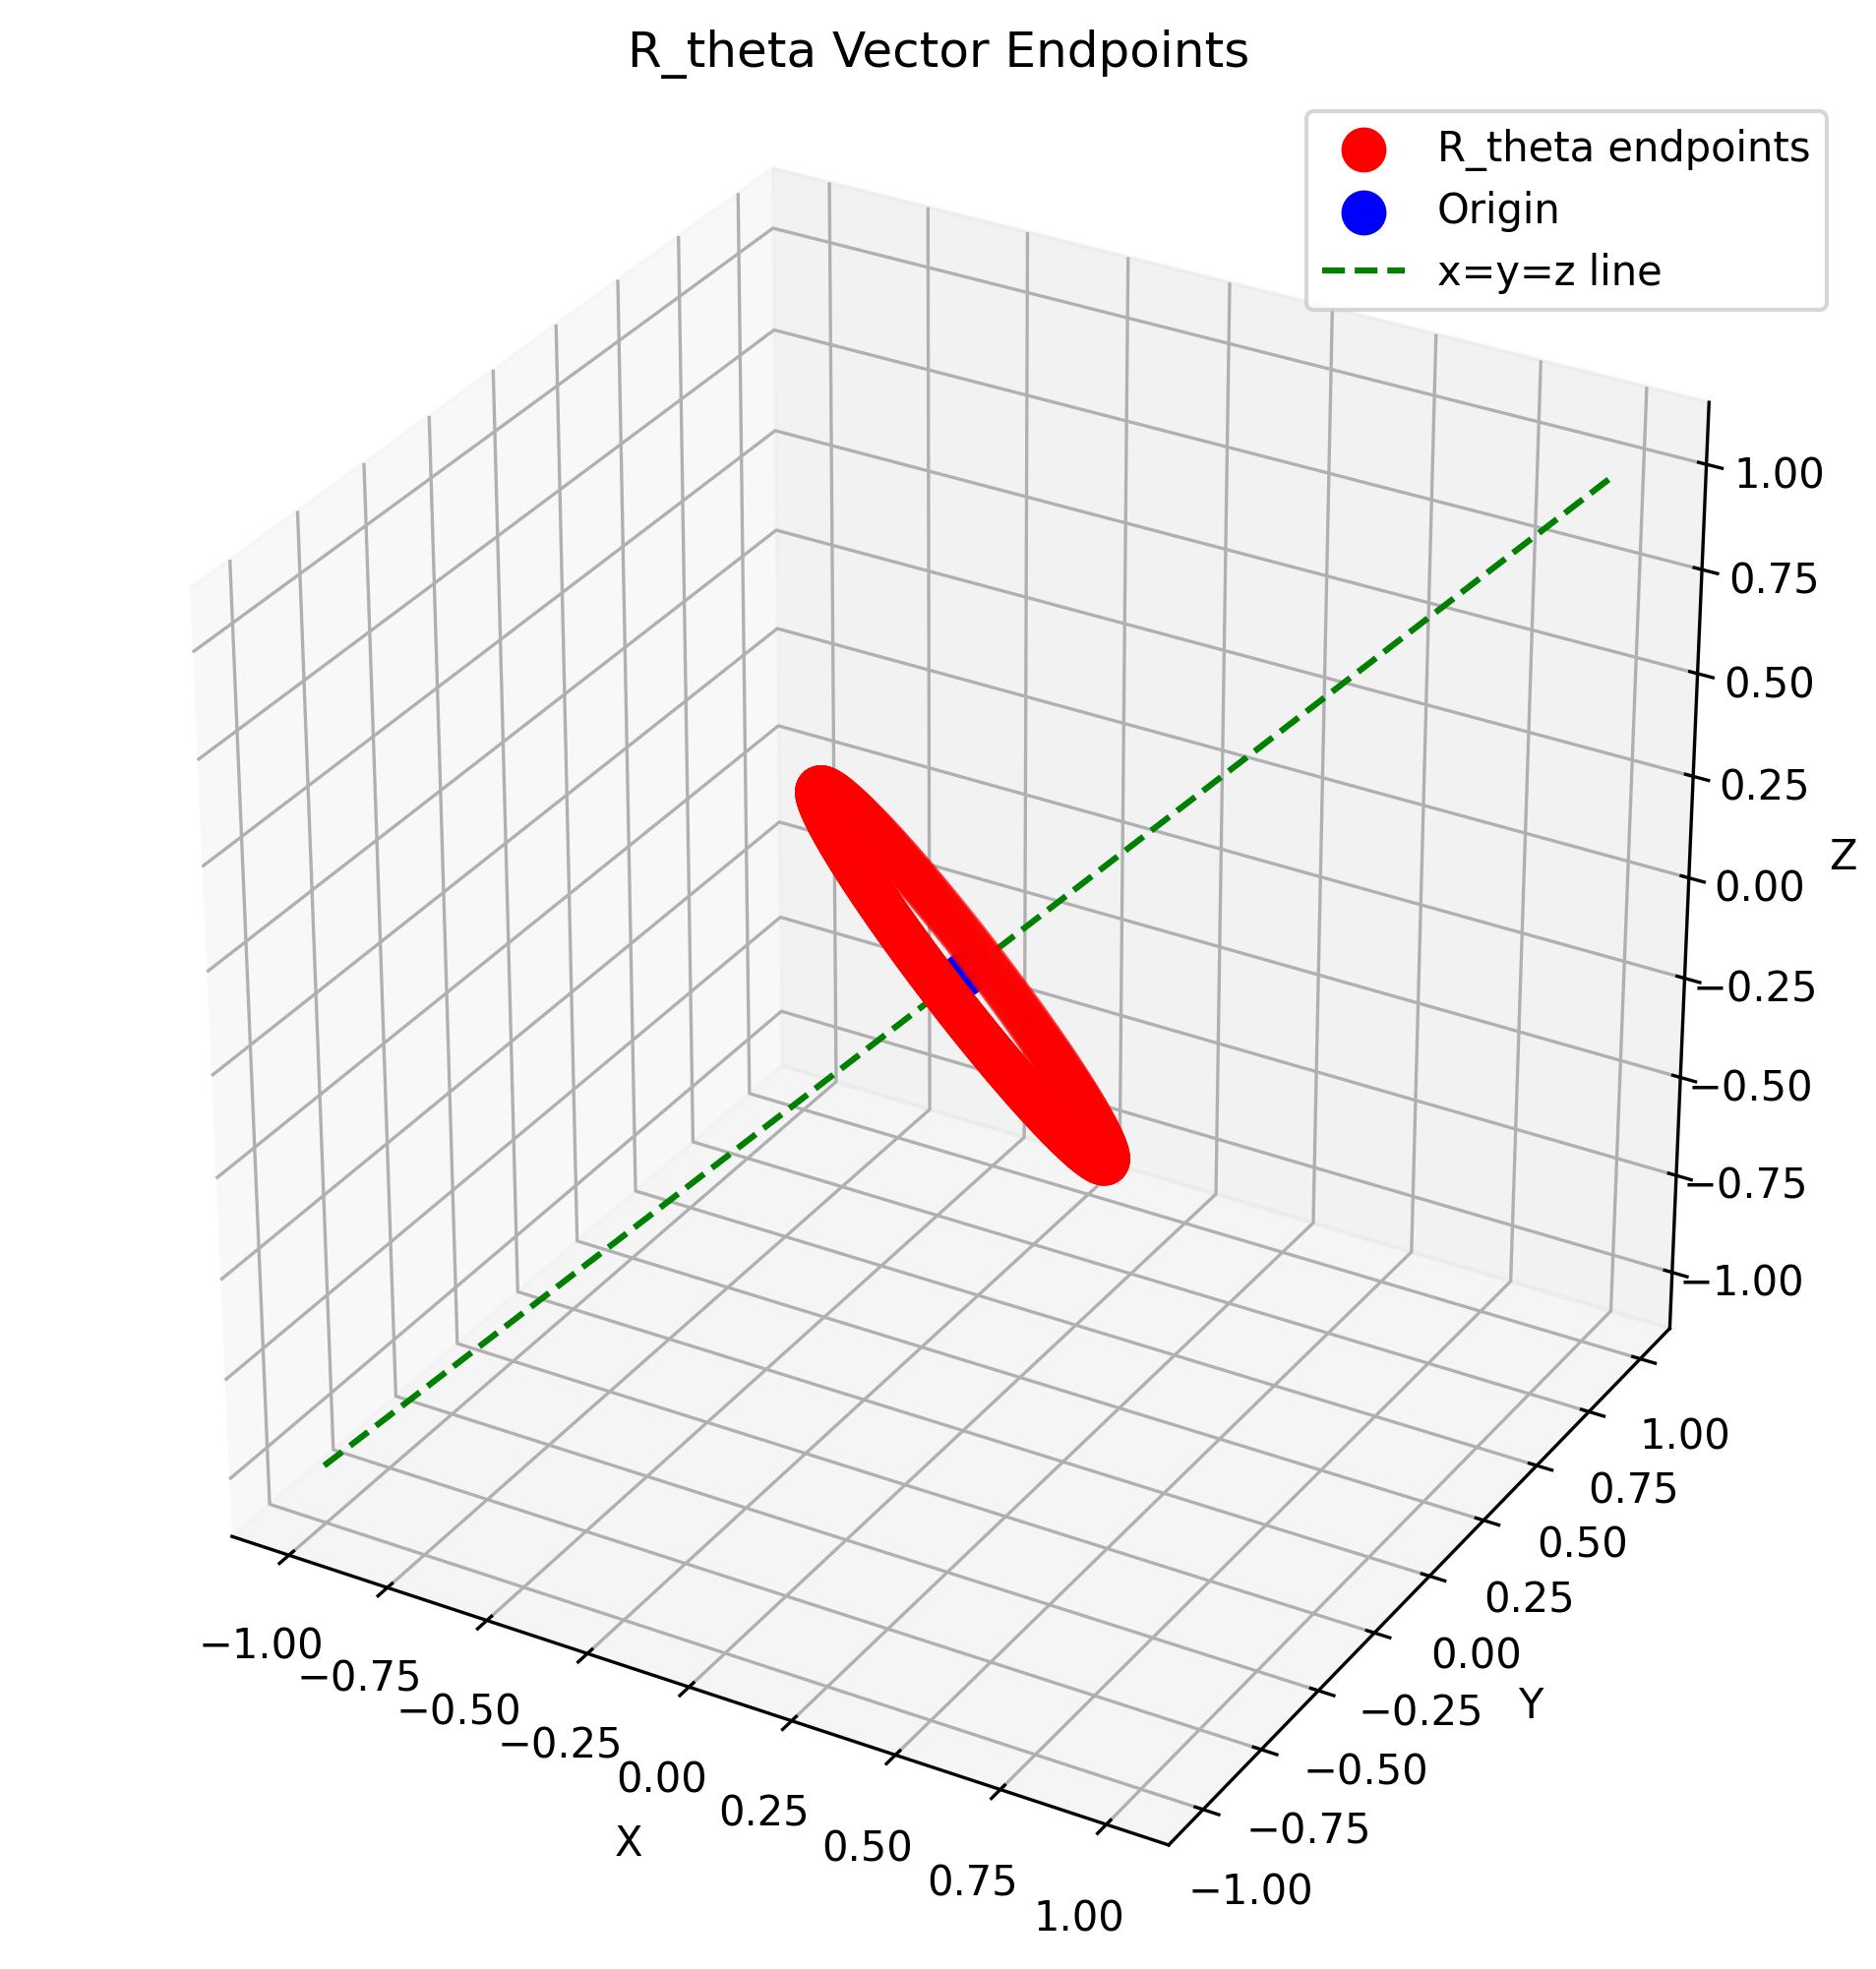
\includegraphics[width=0.8\textwidth]{../example_use/arrowhead_matrix/results/plots/r_vectors_3d.png}
    \caption{R vectors forming a circle in 3D space (72 points, 0-360° in 5° increments)}
    \label{fig:r_vectors_3d}
\end{figure}

\subsection{File Organization}

The output files from the arrowhead matrix visualization are organized into subdirectories based on their file types:

\begin{itemize}
    \item \textbf{plots/}: Contains all PNG image files
    \item \textbf{numpy/}: Contains all NumPy data files (.npy)
    \item \textbf{text/}: For text files
    \item \textbf{csv/}: For CSV files
\end{itemize}

This organization makes it easier to find and work with the files, especially when generating a large number of plots and data files.
